\begin{center}
    {\Large \bf{Appendix}}\\ \vspace{1em}
\end{center}
The Appendix is structured as follows: In Appendix~\ref{sec:proofs}, we gather the proofs related to the properties of $\be(G)$ and $\hbar$-perfect graphs in Appendix~\ref{sec:proofs1}, the $\hbar$-perfectness of $G_7$ and $G_{15}$ in Appendix~\ref{ssec:hper2}, the relation between the length of representation and the adjacency matrix in Appendix~\ref{sec:proofs2}, and the convergence of generalized beta numbers in Appendix~\ref{ssec:gbn}. In Appendix~\ref{sec:numtools}, we provide the details of the new hierarchy based on state polynomial optimization in Appendix~\ref{ssec:spo}, its combination with a see-saw method in Appendix~\ref{ssec:seesaw_state}, the numerical results on all graphs up to $9$ vertices in Appendix~\ref{ssec:typical}, the further application of this hierarchy in shadow tomography in Appendix~\ref{ssec:hierprop}, and the asymptotic prevalence of $\hbar$-perfectness in Appendix~\ref{ssec:asym}. In Appendix C, we supplement the details of the applications. Especially, Appendix~\ref{ssec:entanglement} discusses entanglement detection and estimation, Appendix~\ref{ssec:tomography} analyzes the sample complexity of shadow tomography, Appendix~\ref{ssec:ground} focuses on ground state energy problems, and Appendix~\ref{ssec:alpha} explores the quantum encoding of the independence number.



\section{Proofs related to beta number and $\hbar$-perfectness}
\label{sec:proofs}

\subsection{\texorpdfstring{Proposition 1, Theorem 1 and Theorem 2, Properties 1 to 6}{}}\label{sec:proofs1}
\setcounter{theorem}{0}
\setcounter{proposition}{0}
\begin{proposition}\label{thm:beta}
For given $G$ as a frustration graph, any realization ${\cal S}$ leads to the same set  defined as
	\begin{equation}
		\be(G) \coloneqq \conv(\downarrow\hspace{-0.3em} {\cal Q}({\cal S})) \cap \mathbb{R}_+^n,
	\end{equation}
    where $\downarrow\hspace{-0.3em} T \coloneqq \{x|\exists y \in T\ s.t.\ x_i\le y_i\}$ for a given set $T$.
	Besides, $\beta(G,w) = \max_{v\in \be(G)} \sum_i w_i v_i$, $\forall w\in \mathbb{R}_+^n$.
\end{proposition}
\begin{proof}
    For a given graph $G$ and any two realizations ${\cal S}$ and ${\cal S}'$, let 
    \begin{equation}
        T = \conv(\downarrow\hspace{-0.3em} {\cal Q}({\cal S})) \cap \mathbb{R}_+^n,\ 
        T' = \conv(\downarrow\hspace{-0.3em} {\cal Q}({\cal S}')) \cap \mathbb{R}_+^n.
    \end{equation}
    By definition, both $T$ and $T'$ are convex sets. If there is a point $v \in T'\setminus T$, then there exists a hyperplane to separate $v$ from $T$ in the way that
    \begin{equation}\label{seq:tv}
        \max_{u\in T}\sum_i w_i u_i  < \sum_i w_i v_i,
    \end{equation}
    where $w$ is the norm vector of the corresponding hyperplane.

    Notice that all the elements  $v$ are nonnegative. Hence,
    \begin{equation}\label{seq:ww1}
        \sum_i w_i v_i \le \sum_i w^+_i v_i,
    \end{equation}
    where $w^+_i = \tau_i w_i$ with $\tau_i = \max\{0,{\rm sign}(w_i)\}$.

    Similarly,
    \begin{align}
        \max_{u\in T}\sum_i w_i u_i &\le \max_{u\in T}\sum_i w^+_i u_i\nonumber\\
        &= \max_{u\in T}\sum_{i} w_i \tau_{i} u_i\nonumber\\
        &= \max_{u\in T}\sum_{i} w_i (\tau_{i} u_i)\nonumber\\
        &\le \max_{u'\in T}\sum_{i} w_i u'_i,
    \end{align}
    where the last inequality follows from the fact that $u' = (u'_1,\ldots) \in T$ whenever $u \in T$ since $T$ is a downset. 
    This implies that
    \begin{equation}\label{seq:ww2}
        \max_{u\in T}\sum_i w_i u_i = \max_{u\in T}\sum_i w^+_i u_i = \beta(G,w^+).
    \end{equation}
    By combining Eqs.(\ref{seq:tv},\ref{seq:ww1},\ref{seq:ww2}), we conclude that
    \begin{equation}\label{eq:contradiction}
        \beta(G,w^+) < \sum_i w^+_i v_i,
    \end{equation}
    which is a contradiction by noticing that $ \beta(G,w^+) = \max_{v'\in T'} \max_i w^+_i v'_i \ge \sum_i w^+_i v_i$.

    Hence, $T'\subseteq T$, and for the same reason $T\subseteq T'$, which means that $T=T'$ and leads to the quantity $\be(G)$ independent of the realization.
\end{proof}
\begin{theorem}
	For any graph $G$, $\stab(G) \subseteq \be(G)$.
\end{theorem}
\begin{proof}
    Notice that $\be(G)$ and $\stab(G)$ are both convex sets. Besides, $\stab(G) = \downarrow\hspace{-0.3em} \stab(G)$. By replacing $T$ by $\be(G)$ and $T'$ by $\stab(G)$ in the proof of Theorem~\ref{thm:beta}, we arrive at a contradiction as in Eq.~\eqref{eq:contradiction} since $\sum_i w_i^+ v_i \le \alpha(G,w^+) \le \beta(G,w^+)$.
\end{proof}

\setcounter{prop}{0}
\begin{prop}[Fully connected union]
\label{thm:connected_union2}
If $G_1, G_2$ are $\hbar$-perfect and $G$ is the fully connected disjoint union of $G_1$ and $G_2$, then $G$ is also $\hbar$-perfect.
\end{prop}

\begin{proof}[Proof of Property \ref{thm:connected_union2}] 
Denote by $\{A_{i}\}$ any realization of $G$, and $V_1, V_2$ the vertex sets of $G_1$ and $G_2$. 
Notice that for any nonnegative weight vector $w$ we have
\begin{align}
      \sum_{i\in V_k} w_i \mean{A_i}^2 &= \max_{\rho}\mean{\sum_{i\in V_k} \sqrt{w_{i}}  x_{i} A_{i}}_{\rho}^2 \nonumber\\
      &\le \max_{\rho} \lambda_k^2 \mean{B_k}_{\rho}^2,
\end{align}
where $B_k = \sum_{i\in V_k} \sqrt{w_{i}}  x_{i} A_{i}/ \lambda_k$, $(x_i)_{i\in V_k}$ is the normalized vector of $\left(\sqrt{w_{i}} \mean{A_{i}}\right)_{i\in V_k}$, and $\lambda_k$ is the maximal eigenvalue of $\sum_{i\in V_k} \sqrt{w_{i}}x_{i}A_{i}$.

By definition, $\{B_1, B_2\} = 0$. Hence,
\begin{align}
      \beta(G,w) &= \sum_{i\in V_1} w_i \mean{A_i}^2 + \sum_{i\in V_2} w_i \mean{A_i}^2 \nonumber\\
      &\le \max_{\rho} \left[\lambda_1^2 \mean{B_1}_{\rho}^2 + \lambda_2^2 \mean{B_2}_{\rho}^2\right]\nonumber\\
      &\le \max_k \lambda_k^2.
\end{align}
However,
\begin{equation}
      \max_k \lambda_k^2 \le \max_k \alpha(G_k,(w_i)_{i\in V_k}) = \alpha(G,w),
\end{equation}
where the first inequality is from the facts that
\begin{equation}
    \lambda_k^2 \le \sum_{i\in V_k} w_i \mean{A_i}^2 \le \beta(G_k,(w_i)_{i\in V_k}),
\end{equation}
and $G_1, G_2$ are $\hbar$-perfect. The last equality is from the assumption that $G$ is the fully connected disjoint union of $G_1$ and $G_2$.
\end{proof}

\begin{prop}[Fully disconnected union]
\label{thm:disconnected_union2}
If $G_1, G_2$ are $\hbar$-perfect and $G$ is the fully disconnected disjoint union of $G_1$ and $G_2$, then $G$ is also $\hbar$-perfect.
\end{prop}
\begin{proof}[Proof of Property \ref{thm:disconnected_union2}]
The proof is similar to the one of Property~\ref{thm:connected_union2}. The difference is that in this case, $ [B_1,B_2] =0$ which leads to 
    \begin{equation}
        \beta(G,w) = \sum_k \lambda_k^2 \le \sum_k \alpha(G_k, (w_i)_{i\in V_k}) = \alpha(G,w).
    \end{equation} 
\end{proof}

\begin{prop}[Induced subgraphs]
\label{thm:subgraph2}
    For a $\hbar$-perfect graph $G$, if graph $G'$ is an induced subgraph of $G$ with the vertex set $V'$, then $G'$ is also $\hbar$-perfect.
\end{prop}
\begin{proof}[Proof of Property \ref{thm:subgraph2}] 
    For any nonnegative weight $w'$ of $G'$, denote by $w$ the weight of $G$, where $w_i = w'_i$ if $i \in V'$, otherwise $w_i = 0$. By definition, $w$ is a nonnegative weight of $G$. Consequently,
    \begin{align}
        \beta(G',w') = \beta(G,w) = \alpha(G,w) = \alpha(G',w'),
    \end{align}
    which implies that $G'$ is also $\hbar$-perfect.
\end{proof}

\begin{prop}[Lexicographic product] \label{thm:product2}
  For two given $\hbar$-perfect graphs $G_1$ and $G_2$, denote by $G = G_1[G_2]$ the lexicographic product~\cite{sabidussi1961} of $G_1$ and $G_2$, then $G$ is also $\hbar$-perfect.
\end{prop}
\begin{proof}[Proof of Property \ref{thm:product2}]
  Let $\{A_{ij}\}$ be any realization of $G$, where $A_{ij}$ represents the vertex in $G$ which corresponds to $i$ in $G_1$ and $j$ in $G_2$. 
  For any nonnegative weight $w = (w_{ij})_{ij}$, let $\bar{A}_i = \sum_j \sqrt{w_{ij}}x_{ij}A_{ij}/\lambda_i$, where $(x_{ij})_{j}$ is the normalized vector of $\left(\sqrt{w_{ij}} \mean{A_{ij}}\right)_{j}$, and $\lambda_i$ is the maximal eigenvalue of $\sum_j \sqrt{w_{ij}}x_{ij}A_{ij}$.

  By definition,
  \begin{align}\label{eq:product_upper_bound}
    \beta(G,w) &= \max_{\rho} \sum_{i} \sum_j w_{ij}\mean{A_{ij}}_{\rho}^2\nonumber\\
%             &\le \sum_i \max_{\rho, \{A_{ij}\} \in \mathcal{S}(G)} \sum_j \mean{A_{ij}}_{\rho}^2\\
             &= \max_{\rho}\sum_i \mean{\sum_j \sqrt{w_{ij}}  x_{ij} A_{ij}}_{\rho}^2\nonumber\\
             &= \max_{\rho}\sum_i \lambda_i^2 \mean{\bar{A}_i}_{\rho}^2\nonumber\\
             &\le \max_{\rho}\sum_i \beta(G_2, (w_{ij})_j) \mean{\bar{A}_i}_{\rho}^2\nonumber\\
             &\le \beta(G_1, (\beta(G_2, (w_{ij})_j))_i )\nonumber\\
             &= \alpha(G_1, (\alpha(G_2, (w_{ij})_j))_i )\nonumber\\
             &= \alpha(G,w),
  \end{align}
  where the first inequality in the forth line is from the following fact: 
  \begin{equation}
    \lambda_i^2 = \max_{\rho}\mean{\sum_j \sqrt{w_{ij}} x_{ij} A_{ij}}_{\rho}^2 \le \beta(G_2, (w_{ij})_j).
  \end{equation}
  The second inequality in the fifth line relies on the fact~\cite{xu2023bounding} that $\{\bar{A}_i\} = \{ U (B_i\otimes D_i) U^\dagger\}$ for some unitary $U$, where $B_i$ is the shortest realization of $G_1$ and $D_i$ is diagonal with the absolute values of diagonal elements no more than $1$.
  In the second last equality, we have made use of the fact that both $G_1$ and $G_2$ are $\hbar$-perfect.
  However, $\beta(G,w)$ is always not less than $\alpha(G,w)$. Hence, $\beta(G,w) = \alpha(G,w)$.
\end{proof}

\begin{prop}[Splitting of vertices]
\label{thm:splitting2}
For a $\hbar$-perfect graph $G$, if the graph $G'$ is obtained from $G$ by splitting one vertex, then $G'$ is also $\hbar$-perfect.
\end{prop}
\begin{proof} {Proof of Property \ref{thm:splitting2}.}
Notice that $G'$ is an induced subgraph of the lexicographic product of $G$ and the complete graph $K_2$ with two vertices. Hence, the $\hbar$-perfectness of $G'$ follows from Properties~\ref{thm:subgraph2} and \ref{thm:product2}.
\end{proof}

\begin{prop}[Copying of vertices]
\label{thm:copy2}
For a $\hbar$-perfect graph $G$, if the graph $G'$ is obtained from $G$ by copying one vertex, then $G'$ is also $\hbar$-perfect.
\end{prop}

\begin{proof} {Proof of Property \ref{thm:copy2}.}
    Without loss of generality, we label the vertex which has been copied and its copy with $n$ and $n+1$, respectively, where $n$ is the size of $G$. Furthermore, we take the realization $\{A_i\}_{i=1}^n \cup \{A_n\}$ of $G'$, where $\{A_i\}_{i=1}^n$ is one of $G$. For any nonnegative weight vector $w$ for $G'$, we have
    \begin{equation}
        \max_{\rho} \sum_{i=1}^{n+1} w_i \mean{A_i}^2_{\rho} = \max_{\rho} \sum_{i=1}^n \tilde{w}_i \mean{A_i}^2_{\rho},
    \end{equation}
    where $\tilde{w}_i = w_i$ for $i=1, \ldots, n-1$ and $\tilde{w}_n = w_n + w_{n+1}$.
    This implies that
    \begin{align}
        \beta(G,w)  = \beta(G,\tilde{w}) = \alpha(G,\tilde{w}) = \alpha(G,w).
    \end{align}
\end{proof}




\begin{theorem}[Perfect and $h$-Perfect graphs]\label{thm:perfect2}
    Any perfect graph and any $h$-perfect graph is $\hbar$-perfect. That is,
    \begin{align}
      \text{perfect }  \Rightarrow \text{$h$-perfect }  \Rightarrow \text{$\hbar$-perfect }.
    \end{align}
    In addition, odd cycles are all $h$-perfect graphs. 
\end{theorem}
\begin{proof}
As stated in the main text, for a given graph $G$, if all the facets of $\stab(G)$ can be grouped into the following three classes:
    \begin{enumerate}
        \item $x_i \ge 0$, for $i$ in the vertex set of $G$;
        \item $\sum_{i\in K} x_i \le 1$, for $K$ a clique in $G$;
        \item $\sum_{i\in C} x_i \le a$, for $C$ an odd-cycle in $G$ with $2a+1$ vertices with $a$ being an integer,
     \end{enumerate}
    then it is $h$-perfect~\cite{chvatal1975certain,fonlupt1982transformations}. 
If and only if the third class vanishes as well, the graph is perfect~\cite{chvatal1975certain}. Thus, it is clear that perfect graphs are always $h$-perfect.

    For a given $h$-perfect graph $G$, to prove its $\hbar$-perfectness is equivalent to prove that any point $x$ in $\be(G)$ satisfies all the constraints corresponding to facets of $\stab(G)$. 
    By definition, $\beta(G,w) \ge 0$ for any nonnegative weight vector $w$, hence $x_i \ge 0$ holds always.
    Since $\beta(K) = 1$ for any $K$ a clique in $G$, we know that $\sum_{i\in K} x_i \le 1$. Similarly, $\beta(C) = a$ for any odd-cycle $C$ in $G$ with $2a+1$ vertices~\cite{xu2023bounding}, which implies that $\sum_i x_i \le a$.
\end{proof}

\subsection{$\hbar$-perfectness of $G_7$ and $G_{15}$}
\label{ssec:hper2}
Among all graphs on $7$ vertices there are two whose $\hbar$-perfectness cannot be determined using the properties in the previous section. One of them is $\bar{C}_7$, which is known to be $\hbar$-imperfect. Another one is shown in Fig.~\ref{fig:g7}, which is named as $G_7$ here and we prove that it is $\hbar$-perfect. Notice that all the graphs with no more than $6$ vertices are $\hbar$-perfect, $G_7$ has only one facet whose norm vector contains no zero, and this norm vector is full of $1$. To prove the $\hbar$-perfectness of $G_7$, it is sufficient to prove $\beta(G_7)=\alpha(G_7)=2$.
\begin{proof}[Proof of $\beta(G_7)=2$]
\begin{figure}[ht]
    \centering
    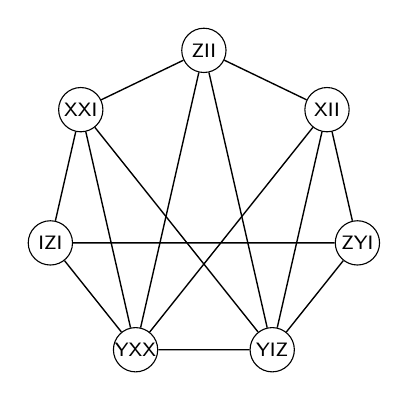
\begin{tikzpicture}[scale=0.8,every node/.style={draw, circle,minimum size=16, inner sep=-2, font=\sffamily\scriptsize}]
  \foreach \i/\lab in {0/ZII,1/XII,2/ZYI,3/YIZ,4/YXX,5/IZI,6/XXI} {
    \node (v\i) at ({90 - \i*360/7}:2.5cm) {\lab};
  }
  \foreach \a/\b in {0/1,1/2,2/3,3/4,4/5,5/6,6/0,0/3,0/4,1/3,1/4,6/3,6/4,2/5} {
    \draw[line width=0.5] (v\a) -- (v\b);
  }
\end{tikzpicture}
    \caption{ \label{fig:ZweiGraphenUndEineTabelle2}The graph $G_7$.}
    \label{fig:g7}
\end{figure}

A standard realization $(S_i)_{i=1}^7$ of $G_7$ in the order as in Fig.~\ref{fig:ZweiGraphenUndEineTabelle2} is
\begin{align}
    Z_1, X_1X_2, Z_2, Y_1X_2X_3, Y_1Z_3, Z_1Y_2, X_1.
\end{align}
For any real unit vector $\vec{w} = (w_i)_{i=1}^7$, we can find out the maximal singular value $\delta(\vec{w})$ of $\sum_i w_i S_i$ analytically as a function of $\vec{w}$. More explicitly,
\begin{align}
    \Delta(\vec{w}) \coloneqq\frac{[\delta(\vec{w})^2-1]^2}{4} = &w_1^2 (w_3^2+w_6^2)+w_3^2 (w_5^2+w_7^2) +w_6^2 (w_2^2+w_4^2)+w_2^2 w_7^2 +2 |w_3 w_6| \sqrt{w_5^2 (w_2^2+w_4^2)+w_4^2 w_7^2}.
\end{align}

Define 
\begin{equation}
    x_0 = \omega_1^2, x_1 = \omega_3^2, x_2 = \omega_6^2, y_1 = \omega_5^2+ \omega_7^2, y_2 = \omega_2^2+ \omega_4^2, z = \sqrt{y_1 y_2-\omega^2 \omega^4}.
\end{equation}
Then we have
\begin{equation}\label{eq:complicated}
   \Delta(\vec{w}) =  x_0 x_1+ x_0 x_2 + x_1 y_1 + x_2 y_2 + 2\sqrt{x_1 x_2}z+y_1y_2-z^2,
\end{equation}
where $x_0 + x_1 + x_2 + y_1 + y_2 = 1$ and $0 \leq z \leq \sqrt{y_1 y_2}$.

Since the right-hand side of Eq.~\eqref{eq:complicated} is a quadratic form in $z$, its maximum is achieved when $z = \min \{\sqrt{y_1 y_2}, \sqrt{x_1x_2} \}$.

We consider the first case that  $y_1 y_2 \leq x_1 x_2$. In this case, by setting $z = \sqrt{y_1y_2}$, we have
\begin{align}
     \Delta(\vec{w}) &= x_0 x_1+ x_0 x_2 + x_1 y_1 + x_2 y_2 + 2\sqrt{x_1 x_2 y_1 y_2}\nonumber\\
     &\le x_0 x_1+ x_0 x_2 + x_1 y_1 + x_2 y_2 + x_1 y_2 + x_2 y_1\nonumber\\
     &= (x_0 + y_1 + y_2)(x_1 + x_2)\nonumber\\
     &\le [(x_0 + y_1 + y_2) + (x_1 + x_2)]^2/4\nonumber\\
     &=1/4.
\end{align}
In the second case that  $y_1 y_2 \geq x_1 x_2$, by setting $z = \sqrt{x_1x_2}$ we have
\begin{align}
     \Delta(\vec{w}) &= x_0 x_1+ x_0 x_2 + x_1 y_1 + x_2 y_2 + x_1 x_2 + y_1 y_2.
\end{align}
For any given $x_1, x_2$ and $y_1$, the value of $x_0 + y_1$ is also fixed and $\Delta(\vec{w})$ is a linear function of $x_0$ and $y_1$. Hence, the maximum of $\Delta(\vec{w})$ is achieved either when $x_0 = 0$ or $y_1=x_1x_2/y_2$, where the second situation is covered by the previous case. For $x_0 = 0$, 
\begin{align}
     \Delta(\vec{w}) &= x_1 y_1 + x_2 y_2 + x_1 x_2 + y_1 y_2 = (x_1 + y_2) (x_2 + y_1)  \le 1/4.
\end{align}
In summary, we have proven that $\Delta(\vec{w}) \le 1/4$ and consequently $\delta(\vec{w})^2 \le 2$, which implies that $\beta(G_7) \le 2$. Since $\beta(G_7) \ge \alpha(G_7) = 2$, we conclude that $\beta(G_7) = 2$.
\end{proof}
\begin{figure}[htpb]
	\centering
	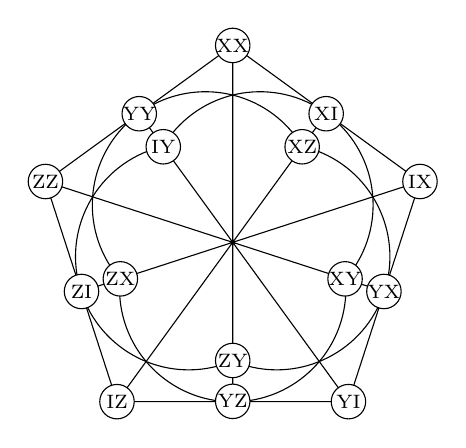
\begin{tikzpicture}[scale=1.25]
\foreach \i in {1,...,5} {
    \pgfmathsetmacro{\angleA}{72*(\i-1) + 18}  % Outer pentagon: 2π/5*(i-1) + π/10
    \pgfmathsetmacro{\angleB}{72*(\i-1) - 18}  % Middle and inner: 2π/5*(i-1) - π/10  
    \coordinate (ps\i) at (\angleA:2); 
    \coordinate (ps2\i) at (\angleB:1.615);  
    \coordinate (ps3\i) at (\angleB:1.2);}
\draw (ps1) -- (ps2) -- (ps3) -- (ps4) -- (ps5) -- cycle;
\draw (ps1) -- (ps24) (ps2) -- (ps25) (ps3) -- (ps21) (ps4) -- (ps22) (ps5) -- (ps23);
\foreach \i in {1,...,5} {
    \pgfmathsetmacro{\rotangle}{72*(\i-1)}
    \begin{scope}[rotate=\rotangle]
        \draw (0, -0.47) + (180:1.15) arc (180:360:1.15);
    \end{scope}}
\def\labels{{"IX", "XX", "ZZ", "IZ", "YI", "YX", "XI", "YY", "ZI", "YZ", "XY", "XZ", "IY", "ZX", "ZY"}}
\foreach \i in {1,...,5} {
    \filldraw[fill=white, draw=black] (ps\i) circle (0.175);
    \pgfmathparse{\labels[\i-1]}
    \node[font=\scriptsize, inner sep=0.5pt] at (ps\i) {\pgfmathresult}; 
    \filldraw[fill=white, draw=black] (ps2\i) circle (0.175);
    \pgfmathparse{\labels[\i+4]}
    \node[font=\scriptsize, inner sep=0.5pt] at (ps2\i) {\pgfmathresult};
    \filldraw[fill=white, draw=black] (ps3\i) circle (0.175);
    \pgfmathparse{\labels[\i+9]}
    \node[font=\scriptsize, inner sep=0.5pt] at (ps3\i) {\pgfmathresult};}
\end{tikzpicture}
	\caption{The complementary graph of $G_{15}$ where all the vertices on the same line or half-circle are connected and the operators on the adjacent vertices commute with each other.}
	\label{fig:g15c}
\end{figure}
Denote by $G_{15}$ the frustration graph of all the $15$ Pauli strings with length $2$ except the identity, then $G_{15}$ is $\hbar$-perfect.
\begin{proof}[Proof of $\hbar$-perfectness of $G_{15}$]
	Due to the high symmetry in $G_{15}$ as illustrated in Fig.~\ref{fig:g15c}, all the facets of $G_{15}$ can be classified into 
	\begin{enumerate}
		\item $x_i \ge 0$,
		\item $\sum_{i\in C} x_i \le 1$, for all cliques $C$,
		\item $\sum_{i\in G'} x_i \le 2$, where $G'$ is any subgraph  isomorphic to the one without vertices labeled by $\{\id X, \id Z, XY, ZY, YY\}$. 
	\end{enumerate}
	For the first two classes, the corresponding beta number equals the independence number naturally. For the third class, the beta number is also $2$ as the independence number, which has been proven in Ref.~\cite{xu2023bounding}. Hence, $G_{15}$ is $\hbar$-perfect by definition.

\end{proof}


\subsection{Length of the realization of a frustration graph}\label{sec:proofs2}
\begin{theorem}\label{thm:minlen}
Let $G$ be a frustration graph with an adjacency matrix $A$.  Then the length of Pauli strings in any realization of $G$ is no less than ${\operatorname{rank}_{\mathbb{F}_2}(A)}/2$  with $\operatorname{rank}_{\mathbb{F}_2}(A)$ being the rank of $A$ over the field $\mathbb{F}_2$, which is achieved by the standard realization~\cite{xu2023bounding}.
\end{theorem}

We first notice that each realization $\{S_i\}_i$ with length $t$ of $G$ corresponds to a collection of complete tripatite graphs $T_1, \ldots, T_t$, in the way that $T_k$ is the frustration graph of $\{S_{i,k}\}_i$ with $S_{i,k}$ the $k$-th Pauli matrix of $S_i$.
In addition, $\{S_i, S_j\} = 0$ if and only if there is an odd number of $k$ such that $\{S_{i,k}, S_{j,k}\} = 0$. Consequently,
\begin{equation}\label{eq:decompA}
A = A(T_1) \oplus A(T_2) \oplus \cdots \oplus A(T_t),
\end{equation}
where $\oplus$ is modulo $2$, i.e., in the field $\mathbb{F}_2$.

Denote by $\mathrm{tp}_{\oplus}(G)$ the minimum number $t$ of complete tripartite graphs $T_1, \ldots, T_t$ satisfying Eq.~\eqref{eq:decompA}.
Clearly, $\mathrm{tp}_{\oplus}(G)$ is the shortest length of Pauli strings in any realization, which is thus the length of Pauli strings in the standard realization. Then we only need to prove that $\mathrm{tp}_{\oplus}(G)$ is given by half the $\mathbb{F}_2$-rank of the adjacency matrix $A$, for which we need the following facts.
\begin{lemma}[Ref.~\cite{Delsarte1975AlternatingBF} Lemma~10]\label{lm:standsymp}
	Any skew-symmetric matrix $A$ of order $n$ over the field $\mathbb{F}_q$ has even rank. If $\operatorname{rank}_{\mathbb{F}_q}(A) = r = 2k$, there exists a nonsingular matrix $L$ such that the transformed matrix $L^\top A L$ takes the canonical form $B$:
\begin{equation}
	L^\top A L = B = \bigoplus_{i=1}^k J, \quad \text{where } J = \begin{pmatrix} 0 & 1 \\ 1 & 0 \end{pmatrix}.
\end{equation}
\end{lemma}

\begin{lemma}\label{lm:triadj}
The matrix $M = u v^\top \oplus v u^\top$ over $\mathbb{F}_2$, for any $u, v \in \mathbb{F}_2^n$, is the adjacency matrix of a complete tripartite graph together with other isolated vertices.
\end{lemma}
\begin{proof}
Partitioning the vertex set $V$ based on the supports of $u$ and $v$ into $V_A = \{p: u_p=1, v_p=0\}$, $V_B = \{p: u_p=0, v_p=1\}$, $V_C = \{p: u_p=1, v_p=1\}$, and $V_D = \{p: u_p=0, v_p=0\}$, a case analysis shows that the entry $M_{pq} = u_p v_q \oplus v_p u_q$ is 1 if and only if $p$ and $q$ belong to different sets among $V_A, V_B, V_C$. This corresponds precisely to the adjacency matrix of the complete tripartite graph $K_{V_A, V_B, V_C}$ together with the isolated vertices in $V_D$.
\end{proof}

\begin{lemma}\label{lm:trirank}
For any complete tripartite graph $T$, it holds that ${\operatorname{rank}_{\mathbb{F}_2}(A(T)) \le 2}$.
\end{lemma}
\begin{proof}
Let $T$ be a complete tripartite graph with vertex sets $A, B, C $, whose adjacency matrix $A(T)$ over $\mathbb{F}_2$ is defined in the way that
 $(A(T))_{ij} = 1$ if $i$ and $j$ belong to different parts among $A, B, C $, and $(A(T))_{ij} = 0$ otherwise.


Let $n$ be the number of vertices. Define the indicator vectors $\mathbf{1}_A, \mathbf{1}_B, \mathbf{1}_C \in \mathbb{F}_2^n$ as the characteristic vectors of $A, B, C$, respectively.
Then, by definition,
\begin{equation}
A(T) = \mathbf{1}_A \mathbf{1}_B^\top \oplus \mathbf{1}_B \mathbf{1}_A^\top \oplus \mathbf{1}_A \mathbf{1}_C^\top \oplus \mathbf{1}_C \mathbf{1}_A^\top \oplus \mathbf{1}_B \mathbf{1}_C^\top \oplus \mathbf{1}_C \mathbf{1}_B^\top.
\end{equation}
Define $u = \mathbf{1}_A \oplus \mathbf{1}_C,  w = \mathbf{1}_B \oplus \mathbf{1}_C$, the direct calculation leads to
$A(T) = u w^\top \oplus w u^\top$. That is, $A(T)$ is the sum of two rank-1 matrices modulo $2$. Therefore,
$\operatorname{rank}_{\mathbb{F}_2}(A(T)) \le 2.$
\end{proof}

\begin{proof}
Let $r = \operatorname{rank}_{\mathbb{F}_2}(A) = 2k$ and $t = \mathrm{tp}_{\oplus}(G)$.
We first prove that $t\ge k$.
By definition, $A = \bigoplus_{i=1}^t A(T_i)$. Applying the rank subadditivity property and Lemma~\ref{lm:trirank}, we have
\begin{equation}
2k = \operatorname{rank}_{\mathbb{F}_2}(A) \le \sum_{i=1}^t \operatorname{rank}_{\mathbb{F}_2}(A(T_i)) \le 2t.
\end{equation}
That is, $k \le t$.

We turn to prove that $t\le k$. Since $A$ is an alternating matrix with $\operatorname{rank}_{\mathbb{F}_2}(A)=2k$, then Lemma~\ref{lm:standsymp} guarantees that $A$ is congruent to $B$ via a nonsingular matrix $L$, i.e., $A = L^{-\top} B L^{-1}$, where 
\begin{equation}
    B = \sum_{i=1}^{k} \left( e_{2i-1} e_{2i}^\top \oplus e_{2i} e_{2i-1}^\top \right),
\end{equation}
with $e_j$ the standard basis vectors.
Defining the vectors $u_i = L^{-\top} e_{2i-1}$ and $v_i = L^{-\top} e_{2i}$, we have
\begin{equation}
    A = \sum_{i=1}^{k} M_i, \quad \text{where } M_i = u_i v_i^\top \oplus v_i u_i^\top.
\end{equation}
By Lemma~\ref{lm:triadj}, each matrix $M_i$ is the adjacency matrix of a complete tripartite graph $T_i$. Therefore, $t\le k$ by the definition of $t$.
\end{proof}
Similarly, denote by $\mathrm{tp}(G)$ the minimum number $t$ of complete tripartite graphs $T_1, \ldots, T_t$ satisfying 
\begin{equation}
A = A(T_1) + A(T_2) + \cdots + A(T_t).
\end{equation}
And denote by $\mathrm{bp}(G)$ the minimum number $t$ of complete bipartite graphs $B_1, \ldots, B_t$ satisfying 
\begin{equation}
A = A(B_1) + A(B_2) + \cdots + A(B_t).
\end{equation}
Then, by definition, 
\begin{equation}
\mathrm{tp}_{\oplus}(G) \le \mathrm{tp}(G) \le \mathrm{bp}(G),
\end{equation}
where the last inequality is due to the fact that any complete bipartite graph can be viewed as a complete tripartite graph with one part being empty.
The number $\mathrm{bp}(G)$ is also known as the biclique partition number~\cite{graham1971addressing} of the graph $G$, which has applications in telephone switching circuitry~\cite{graham1971addressing} and its relation with other graph parameters has been established~\cite{lyu2023finding}. 

Here we have focused on arbitrary frustration graphs representing the anticommutation and commutation relations of Pauli strings. Recently, the concept of frustration graph with weighted edges was proposed for the strings of Weyl-Heisenberg matrices~\cite{Makuta2025FrustrationGF}. It is interesting to see that results similar to Theorem~\ref{thm:minlen} hold also for special kinds of frustration graphs with weighted edges.

\subsection{Convergence of generalized beta numbers}
\label{ssec:gbn}
\begin{proposition}
%\label{prop:convergence_generalized_beta}
Given a graph $G$, as $k$ goes to infinity, $\beta(G,w,k)$ converges to the weighted independence number $\alpha(G,w)$.
More precisely, for any nonnegative weight vector $w$,
\begin{equation}
	\lim_{k\to \infty} \beta(G,w,k) = \alpha(G,w).
\end{equation}    
\end{proposition}
\begin{proof}
To begin, notice that $\beta(G,w,k)$ decreases as $k$ increases since $|\langle S_i\rangle|\le 1$, and $\beta(G,w,k) \ge 0$ by definition.
Thus, $\beta(G,w,k)$ converges, and denote by $\tilde{\alpha}(G,w)$ the limit. 

Besides, $\{S_i\}_{i\in I}$ is a set of commuting Pauli strings for an independent set $I$ of $G$, which implies that there is a state $\rho$ such that $|\langle S_i\rangle_\rho| = 1$ for $i\in I$ and the other expectation values . Consequently, $\beta(G,w,k)\ge \max_{I} \sum_{i\in I} w_i = \alpha(G,w)$ for any $k$, by the definition of the weighted independence number. Due to the arbitrariness of $k$, we have $\tilde{\alpha}(G,w) \ge \alpha(G,w)$.

If  $\tilde{\alpha}(G,w)$ is strictly larger than $\alpha(G,w)$, there exists $\epsilon > 0$ such that $\tilde{\alpha}(G,w) \ge \alpha(G,w) + \epsilon$.
For each $k$, denote by $\Lambda_k$ the set of states $\rho$ such that $\sum_i w_i |\langle S_i\rangle^k_\rho| \ge \alpha(G,w)+\epsilon$. By assumption, $\Lambda_k$ is non-empty, closed, and compact. As $|\langle S_i\rangle^k_\rho|$ decreases with $k$, $\Lambda_{k+1} \subseteq \Lambda_k$.
From Cantor's intersection theorem, we know that $\Lambda \coloneqq \cap_{k=1}^\infty \Lambda_k$ is not empty. 

Denote by $\rho$ a state in $\Lambda$, then $\sum_i w_i |\langle S_i\rangle^k_\rho| \ge \alpha(G,w)+\epsilon$ for each $k$ by assumption. Then we have 
\begin{equation}
\begin{aligned}
	\alpha(G,w)+\epsilon & \le
	\lim_{k\to \infty} \sum\nolimits_i w_i |\langle S_i\rangle^k_\rho|\\
			     &= \sum\nolimits_i w_i \big(\lim_{k\to\infty} |\langle S_i\rangle^k_\rho|\big) \\
			     &=\sum\nolimits_{i\in \bar{I}} w_i,
\end{aligned}
\end{equation}
where $\bar{I}$ is the set of all $i$ such that $|\langle S_i\rangle_\rho|=1$. For any $i\not\in \bar{I}$, we have $\lim_{k\to\infty} |\langle S_i\rangle^k_\rho| = 0$ due to $|\langle S_i\rangle_\rho| < 1$.
We claim that $\bar{I}$ must be an independence set, in which case $\sum_{i\in \bar{I}} w_i \le \alpha(G,w)$ results in a contradiction. If $\bar{I}$ is not an independence set, it contains two adjacent vertices $i_1$ and $i_2$. Then $|\langle S_{i_1}\rangle_\rho|$ and  $|\langle S_{i_2}\rangle_\rho|$ cannot be $1$ simultaneously, since the sum of squares of them is no more than $1$, which contradicts the definition of $\bar{I}$. This finishes the proof.
\end{proof}
\section{Numerical methods}\label{sec:numtools}
\subsection{A new hierarchy of SDP relaxations}\label{ssec:spo}
The calculation of the weighted beta number $\beta(G,w)$ can be formulated as a nonlinear optimization problem over the expectations $\langle\cdot\rangle_\rho$:
\begin{equation}\label{eq:spop}
\beta(G,w) \coloneqq \begin{cases}\sup_\rho &\sum_{i=1}^n w_i\langle S_i \rangle_\rho^2\\
\textrm{s.t.}&S_i^2=1,\quad\text{ for }i=1,\ldots,n,\\
&S_iS_j=-S_jS_i,\quad\text{ for }i\sim_{G} j,\\
&S_iS_j=S_jS_i,\quad\text{ for }i\nsim_{G} j,
\end{cases}
\end{equation}
where $i\sim_{G} j$ (reps. $i\nsim_{G} j$) means that the vertices $i$ and $j$ are connected (reps. not connected) in graph $G$.
The problem \eqref{eq:spop} is an instance of state polynomial optimization problems \cite{klep2024state}.
A complete hierarchy of moment-sum-of-Hermitian-squares relaxations was established in \cite{klep2024state} for solving state polynomial optimization problems. We begin by outlining its main idea. Consider letters $\{x_1,\ldots,x_n\}$ and words $u=x_{i_1}\cdots x_{i_t}$ built from these letters. The involution of a word is defined as $(x_{i_1}\cdots x_{i_t})^*=x_{i_t}\cdots x_{i_1}$.
We further consider pseudo-expectations of words $\langle u\rangle=\langle u^*\rangle\in\mathbb{R}$ which behave as scalars. A state monomial in words and pseudo-expectations is of the form $u=u_0\langle u_1\rangle\cdots\langle u_s\rangle$ where $u_0,\ldots,u_s$ are words in $\{x_1,\ldots,x_n\}$. 
When specifying to \eqref{eq:spop}, the constraint $S_i^2=1$ gives rise to $x_i^2=1$ for $i=1,\ldots,n$, and the constraint $S_iS_j=-S_jS_i$ (resp. $S_iS_j=S_jS_i$) for $i\sim_{G} j$ (resp. $i\nsim_{G} j$) gives rise to $x_ix_j=-x_jx_i$ (resp. $x_ix_j=x_jx_i$) for $i\sim_{G} j$ (resp. $i\nsim_{G} j$). Such relations allow us to reduce any word to the normal form $cx_{i_1}\cdots x_{i_t}$ with $i_1<\cdots<i_t$ and $c\in\{-1,1\}$. 

For a state monomial $u=u_0\langle u_1\rangle\cdots\langle u_s\rangle$, its degree is the sum of the lengths of the words $u_i$. Now, given a positive integer $r$, the $r$-th moment matrix $M_r$ is indexed by state monomials of degree at most $r$ and its entry $[M_r]_{u,v}\coloneqq\langle u^*v\rangle$ where $u^*v$ is assumed to be reduced to the normal form. Then, the $r$-th order moment relaxation for \eqref{eq:spop} is given by the following SDP:
\begin{equation}\label{mom}
\lambda_r(G,w)\coloneqq\begin{cases}
\sup &\sum_{i=1}^n w_i\langle x_i\rangle^2\\
\rm{s.t.}&M_r\succeq0,\\
&[M_r]_{1,1}=1,\\
&[M_r]_{u,v}=[M_r]_{a,b}, \text{ if }\langle u^*v\rangle=\langle a^*b\rangle,
\end{cases}
\end{equation}
where $1$ denotes the empty word. It was shown in \cite{klep2024state} that the sequence of upper bounds $(\lambda_r(G,w))_{r\ge1}$ converges monotonically to the optimum of the state polynomial optimization problem \eqref{eq:spop}, i.e., $$\lim_{r\to\infty}\lambda_r(G,w)=\beta(G,w).$$
However, the size of the moment relaxation grows rapidly with the size of the original problem as well as the relaxation order $r$, and so it soon becomes intractable. To circumvent this difficulty, a simplified Lov\'asz-type hierarchy was proposed in \cite{moran2024Uncertainty}, where one considers the reduced moment matrix which is indexed by state monomials of the forms
\begin{gather}
1,\,x_{i}\langle x_{i}\rangle,\,x_{i}x_{j}\langle x_{i}\rangle\langle x_{j}\rangle,\nonumber\\
\cdots\label{lovasz}\\
x_{1}\cdots x_{n}\langle x_{1}\rangle\cdots\langle x_{n}\rangle\nonumber.
\end{gather}
As observed in \cite{moran2024Uncertainty}, the simplified Lov\'asz-type hierarchy may not converge to $\beta(G,w)$ for graphs with $7$ vertices.

Here, to improve the bounds while maintaining scalability, we propose to extend the monomial basis in \eqref{lovasz} by including two-body pseudo-expectations $\langle x_{i}x_{j}\rangle$.
Specifically, we form the monomial basis by selecting state monomials of the forms
\begin{gather}
1,\,x_{i}\langle x_{i}\rangle,x_{i}x_{j}\langle x_{i}\rangle\langle x_{j}\rangle,x_{i}\langle x_{j}\rangle\langle x_{i}x_{j}\rangle,\nonumber\\
x_{i}x_{j}x_{k}\langle x_{i}\rangle\langle x_{j}\rangle\langle x_{k}\rangle,x_{i}x_{j}x_{k}\langle x_{i}x_{j}\rangle\langle x_{k}\rangle,x_{i}x_{k}\langle x_{i}x_{j}\rangle\langle x_{j}\rangle\langle x_{k}\rangle,x_{k}\langle x_{i}x_{j}\rangle\langle x_{i}\rangle\langle x_{j}\rangle\langle x_{k}\rangle,\label{new}\\
\cdots\nonumber
\end{gather}
Note that for $i\sim_{G} j$, it holds that $\langle x_{i}x_{j}\rangle=-\langle x_{j}x_{i}\rangle$ which implies $\langle x_{i}x_{j}\rangle=0$. Thus, we can exclude $\{\langle x_{i}x_{j}\rangle\}_{i\sim_{G} j}$ when constructing the monomial basis \eqref{new}. Moreover, if $\langle u^*v\rangle=-\langle v^*u\rangle$, then we set $\langle u^*v\rangle=\langle v^*u\rangle=0$ in the moment matrix.


Among graphs with $8$ and $9$ vertices, there are $100$ and $2963$ graphs whose $\hbar$-(im)perfectness requires numerical verification, respectively. 
It turns out that by virtue of the new hierarchy we can verify $\hbar$-perfectness for all those graphs with $8$ vertices and verify $\hbar$-perfectness for all but $78$ those graphs with $9$ vertices (up to a $<1\times10^{-5}$ gap between lower and upper bounds). In Table~\ref{tab:g9}, we show the top $12$ graphs that yield the largest gaps. The calculations were performed on a desktop with 128G RAM and {\tt Mosek 10.2} was employed as the underlying SDP solver. Our code for reproducing the results is available at \url{https://github.com/wangjie212/BetaNumber}.

\begin{table}[tbp]
\begin{center}
\def \scale {1.2}
\def \zoom {0.4}
\def \nth {9}
\def \an {360/\nth}
\def \bline {0.1cm}
\def \acolor {black}
\begin{tabular}{c@{\hskip 15pt}c@{\hskip 15pt}c@{\hskip 15pt}c@{\hskip15pt}c@{\hskip15pt}c}
 &\\
  &
 \begin{tikzpicture}[scale=\scale, baseline=\bline]
    \foreach \i in {1,2,...,\nth} {
\coordinate (A\i) at ({-cos(\i*\an)},{sin(\i*\an)}) {};
\node[party, fill=white, scale=\zoom] (A\i) at (A\i) {};
}
\draw (A1)--(A3) (A1)--(A5) (A1)--(A6) (A1)--(A7) (A1)--(A8) (A1)--(A9) (A2)--(A4) (A2)--(A5) (A2)--(A6) (A2)--(A7) (A2)--(A8) (A2)--(A9) (A3)--(A5) (A3)--(A7) (A3)--(A9) (A4)--(A6) (A4)--(A7) (A4)--(A8) (A4)--(A9) (A5)--(A7) (A5)--(A8) (A6)--(A8) (A6)--(A9) (A7)--(A9);
 \end{tikzpicture}
 &
\begin{tikzpicture}[scale=\scale, baseline=\bline]
\foreach \i in {1,2,...,8} {
\coordinate (A\i) at ({-cos(\i*\an)},{sin(\i*\an)}) {};
\node[party, fill=white, scale=\zoom] (A\i) at (A\i) {};
}
\coordinate (A9) at ({-cos(9*\an)},{sin(9*\an)}) {};
\node[draw, party, fill=black, minimum width=1mm, scale=\zoom] (A9) at (A9) {};
\draw (A1)--(A3) (A1)--(A5) (A1)--(A6) (A1)--(A7) (A1)--(A9) (A2)--(A4) (A2)--(A5) (A2)--(A7) (A2)--(A8) (A3)--(A5) (A3)--(A6) (A3)--(A8) (A3)--(A9) (A4)--(A6) (A4)--(A7) (A4)--(A8) (A4)--(A9) (A5)--(A7) (A5)--(A9) (A6)--(A8) (A6)--(A9) (A7)--(A9) (A8)--(A9);
 \end{tikzpicture}
 &
 \begin{tikzpicture}[scale=\scale, baseline=\bline]
    \foreach \i in {1,2,...,8} {
\coordinate (A\i) at ({-cos(\i*\an)},{sin(\i*\an)}) {};
\node[party, fill=white, scale=\zoom] (A\i) at (A\i) {};
}
\coordinate (A9) at ({-cos(9*\an)},{sin(9*\an)}) {};
\node[draw, circle, fill=black, minimum width=1mm, scale=\zoom] (A9) at (A9) {};
\draw (A1)--(A3) (A1)--(A5) (A1)--(A6) (A1)--(A7) (A1)--(A9) (A2)--(A4) (A2)--(A5) (A2)--(A7) (A2)--(A8) (A2)--(A9) (A3)--(A5) (A3)--(A6) (A3)--(A8) (A3)--(A9) (A4)--(A6) (A4)--(A7) (A4)--(A8) (A4)--(A9) (A5)--(A7) (A5)--(A8) (A5)--(A9) (A6)--(A8) (A6)--(A9) (A7)--(A9) (A8)--(A9);
 \end{tikzpicture}
&
 \begin{tikzpicture}[scale=\scale, baseline=\bline]
    \foreach \i in {1,2,...,8} {
\coordinate (A\i) at ({-cos(\i*\an)},{sin(\i*\an)}) {};
\node[party, fill=white, scale=\zoom] (A\i) at (A\i) {};
}
\coordinate (A9) at ({-cos(9*\an)},{sin(9*\an)}) {};
\node[draw, circle, fill=black, minimum width=1mm, scale=\zoom] (A9) at (A9) {};
\draw (A1)--(A3) (A1)--(A5) (A1)--(A6) (A1)--(A7) (A1)--(A9) (A2)--(A4) (A2)--(A5) (A2)--(A7) (A2)--(A8) (A2)--(A9) (A3)--(A5) (A3)--(A6) (A3)--(A8) (A3)--(A9) (A4)--(A6) (A4)--(A7) (A4)--(A8) (A4)--(A9) (A5)--(A7) (A5)--(A8) (A5)--(A9) (A6)--(A8) (A6)--(A9) (A7)--(A9) (A8)--(A9);
 \end{tikzpicture}
\\
 & \\
 $\omega$&$(1, 1, 1, 1, 1, 1, 1, 1, 1)$&$(1, 1, 1, 1, 1, 1, 1, 1, 2)$&$(1, 1, 1, 1, 1, 1, 1, 1, 2)$&$(1, 1, 1, 1, 1, 1, 1, 1, 2)$\\
 $\gamma_{\mathrm{ub}}$ & 2.00048 & 2.00227 & 2.00175&2.00118\\
 see-saw& 2.00000 & 2.00000 & 2.00000&2.00000\\
 $\alpha$ & 2 & 2 & 2&2\\
 &\\
  &
 \begin{tikzpicture}[scale=\scale, baseline=\bline]
    \foreach \i in {1,2,...,8} {
\coordinate (A\i) at ({-cos(\i*\an)},{sin(\i*\an)}) {};
\node[party, fill=white, scale=\zoom] (A\i) at (A\i) {};
}
\coordinate (A9) at ({-cos(9*\an)},{sin(9*\an)}) {};
\node[draw, circle, fill=black, minimum width=1mm, scale=\zoom] (A9) at (A9) {};
\draw (A1)--(A3) (A1)--(A5) (A1)--(A6) (A1)--(A7) (A1)--(A8) (A1)--(A9) (A2)--(A4) (A2)--(A5) (A2)--(A7) (A2)--(A8) (A2)--(A9) (A3)--(A5) (A3)--(A6) (A3)--(A8) (A3)--(A9) (A4)--(A6) (A4)--(A7) (A4)--(A8) (A4)--(A9) (A5)--(A7) (A5)--(A8) (A5)--(A9) (A6)--(A7) (A6)--(A8) (A6)--(A9) (A7)--(A9) (A8)--(A9);
 \end{tikzpicture}
 &
\begin{tikzpicture}[scale=\scale, baseline=\bline]
    \foreach \i in {1,2,...,\nth} {
\coordinate (A\i) at ({-cos(\i*\an)},{sin(\i*\an)}) {};
\node[party, fill=white, scale=\zoom] (A\i) at (A\i) {};
}
\draw (A1)--(A3) (A1)--(A5) (A1)--(A6) (A1)--(A7) (A1)--(A8) (A1)--(A9) (A2)--(A4) (A2)--(A5) (A2)--(A6) (A2)--(A7) (A2)--(A8) (A2)--(A9) (A3)--(A5) (A3)--(A7) (A3)--(A8) (A3)--(A9) (A4)--(A6) (A4)--(A7) (A4)--(A8) (A4)--(A9) (A5)--(A6) (A5)--(A7) (A6)--(A8) (A7)--(A9) (A8)--(A9);
 \end{tikzpicture}
 &
\begin{tikzpicture}[scale=\scale, baseline=\bline]
    \foreach \i in {1,2,...,\nth} {
\coordinate (A\i) at ({-cos(\i*\an)},{sin(\i*\an)}) {};
\node[party, fill=white, scale=\zoom] (A\i) at (A\i) {};
}
\draw (A1)--(A3) (A1)--(A5) (A1)--(A6) (A1)--(A7) (A1)--(A8) (A1)--(A9) (A2)--(A4) (A2)--(A5) (A2)--(A7) (A2)--(A8) (A2)--(A9) (A3)--(A5) (A3)--(A6) (A3)--(A7) (A3)--(A9) (A4)--(A6) (A4)--(A7) (A4)--(A8) (A4)--(A9) (A5)--(A6) (A5)--(A8) (A5)--(A9) (A6)--(A8) (A7)--(A9) (A8)--(A9);
 \end{tikzpicture}
&
\begin{tikzpicture}[scale=\scale, baseline=\bline]
    \foreach \i in {1,2,...,8} {
\coordinate (A\i) at ({-cos(\i*\an)},{sin(\i*\an)}) {};
\node[party, fill=white, scale=\zoom] (A\i) at (A\i) {};
}
\coordinate (A9) at ({-cos(9*\an)},{sin(9*\an)}) {};
\node[draw, circle, fill=black, minimum width=1mm, scale=\zoom] (A9) at (A9) {};
\draw (A1)--(A3) (A1)--(A4) (A1)--(A6) (A1)--(A7) (A1)--(A9) (A2)--(A4) (A2)--(A5) (A2)--(A6) (A2)--(A7) (A2)--(A8) (A2)--(A9) (A3)--(A5) (A3)--(A6) (A3)--(A8) (A3)--(A9) (A4)--(A6) (A4)--(A7) (A4)--(A8) (A4)--(A9) (A5)--(A7) (A5)--(A8) (A5)--(A9) (A6)--(A8) (A6)--(A9) (A7)--(A9) (A8)--(A9);
 \end{tikzpicture}
 \\
 & \\
 $\omega$&$(1, 1, 1, 1, 1, 1, 1, 1, 2)$&$(1, 1, 1, 1, 1, 1, 1, 1, 1)$&$(1, 1, 1, 1, 1, 1, 1, 1, 1)$&$(1, 1, 1, 1, 1, 1, 1, 1, 2)$\\
 $\gamma_{\mathrm{ub}}$ & 2.00056 & 2.00125 & 2.00058&2.00227\\
 see-saw& 2.00000 & 2.00000 & 2.00000&2.00000\\
 $\alpha$ & 2 & 2 & 2&2\\
 &\\
  &
\begin{tikzpicture}[scale=\scale, baseline=\bline]
    \foreach \i in {1,2,...,\nth} {
\coordinate (A\i) at ({-cos(\i*\an)},{sin(\i*\an)}) {};
\node[party, fill=white, scale=\zoom] (A\i) at (A\i) {};
}
\draw (A1)--(A3) (A1)--(A4) (A1)--(A6) (A1)--(A7) (A1)--(A8) (A1)--(A9) (A2)--(A4) (A2)--(A5) (A2)--(A6) (A2)--(A7) (A2)--(A8) (A2)--(A9) (A3)--(A5) (A3)--(A6) (A3)--(A8) (A3)--(A9) (A4)--(A6) (A4)--(A7) (A4)--(A8) (A4)--(A9) (A5)--(A7) (A5)--(A8) (A5)--(A9) (A6)--(A8) (A7)--(A9) (A8)--(A9);
 \end{tikzpicture}
 &
\begin{tikzpicture}[scale=\scale, baseline=\bline]
    \foreach \i in {1,2,...,\nth} {
\coordinate (A\i) at ({-cos(\i*\an)},{sin(\i*\an)}) {};
\node[party, fill=white, scale=\zoom] (A\i) at (A\i) {};
}
\draw (A1)--(A3) (A1)--(A4) (A1)--(A6) (A1)--(A7) (A1)--(A8) (A1)--(A9) (A2)--(A4) (A2)--(A5) (A2)--(A6) (A2)--(A7) (A2)--(A8) (A2)--(A9) (A3)--(A5) (A3)--(A6) (A3)--(A7) (A3)--(A8) (A3)--(A9) (A4)--(A6) (A4)--(A7) (A4)--(A8) (A4)--(A9) (A5)--(A7) (A5)--(A8) (A5)--(A9) (A6)--(A8) (A6)--(A9) (A7)--(A9);
 \end{tikzpicture}
 &
\begin{tikzpicture}[scale=\scale, baseline=\bline]
    \foreach \i in {1,2,...,8} {
\coordinate (A\i) at ({-cos(\i*\an)},{sin(\i*\an)}) {};
\node[party, fill=white, scale=\zoom] (A\i) at (A\i) {};
}
\coordinate (A9) at ({-cos(9*\an)},{sin(9*\an)}) {};
\node[draw, circle, fill=black, minimum width=1mm, scale=\zoom] (A9) at (A9) {};
\draw (A1)--(A3) (A1)--(A4) (A1)--(A6) (A1)--(A7) (A1)--(A8) (A1)--(A9) (A2)--(A4) (A2)--(A5) (A2)--(A6) (A2)--(A7) (A2)--(A8) (A2)--(A9) (A3)--(A5) (A3)--(A6) (A3)--(A7) (A3)--(A8) (A3)--(A9) (A4)--(A6) (A4)--(A7) (A4)--(A8) (A4)--(A9) (A5)--(A7) (A5)--(A8) (A5)--(A9) (A6)--(A8) (A6)--(A9) (A7)--(A9) (A8)--(A9);
 \end{tikzpicture}
 &
 \begin{tikzpicture}[scale=\scale, baseline=\bline]
    \foreach \i in {1,2,...,\nth} {
\coordinate (A\i) at ({-cos(\i*\an)},{sin(\i*\an)}) {};
\node[party, fill=white, scale=\zoom] (A\i) at (A\i) {};
}
\draw (A1)--(A3) (A1)--(A4) (A1)--(A5) (A1)--(A7) (A1)--(A8) (A1)--(A9) (A2)--(A4) (A2)--(A5) (A2)--(A6) (A2)--(A7) (A2)--(A8) (A2)--(A9) (A3)--(A5) (A3)--(A6) (A3)--(A7) (A3)--(A8) (A3)--(A9) (A4)--(A6) (A4)--(A7) (A4)--(A8) (A4)--(A9) (A5)--(A7) (A5)--(A8) (A6)--(A8) (A6)--(A9) (A7)--(A9);
 \end{tikzpicture}
 \\
 & \\
 $\omega$&$(1, 1, 1, 1, 1, 1, 1, 1, 1)$&$(1, 1, 1, 1, 1, 1, 1, 1, 1)$&$(1, 1, 1, 1, 1, 1, 1, 1, 2)$&$(1, 1, 1, 1, 1, 1, 1, 1, 1)$\\
 $\gamma_{\mathrm{ub}}$ & 2.00073 & 2.00062 & 2.00083&2.00094\\
 see-saw& 2.00000 & 2.00000 & 2.00000&2.00000\\
 $\alpha$ & 2 & 2 & 2&2\\
\end{tabular}
\end{center}
\caption{The top $12$ graphs with the largest gaps, where black vertices are of weights $2$. Here, $\gamma_{\mathrm{ub}}$ denotes the upper bound given by SDP relaxations and ``see-saw'' denotes the lower bound given by the see-saw method.}\label{tab:g9}
\end{table}


\subsection{Retrieving an approximately optimal state}\label{ssec:seesaw_state}
After solving the moment relaxation for \eqref{eq:spop}, it is possible to retrieve an approximately optimal state to \eqref{eq:spop} from the SDP solution. Suppose that the length of $S_1,\ldots,S_n$ is $m$ and $\{\langle x_{i}\rangle^2\}_{i=1}^n$ are extracted from the moment matrix. Then, for any binary vector $(a_i)_{i=1}^n\in\{-1,1\}^n$, we consider the following nonlinear SDP:
\begin{equation}\label{extract}
\begin{cases}
\min_{\rho\in\mathbb{S}^{2^m}} &\sum_{i=1}^n \left(\tr(\rho S_i)-a_i\sqrt{\langle x_{i}\rangle^2}\right)^2\\
\rm{s.t.}&\rho\succeq0,\\
&\tr(\rho)=1.\\
\end{cases}
\end{equation}
The objective of \eqref{extract} is a convex quadratic function in $\rho$ and could be solved by SDP solvers, e.g., {\tt COSMO} \cite{Garstka_2021}. In practice, we need to traverse all binary vectors $(a_i)_{i=1}^n$ and solve the corresponding SDPs \eqref{extract} until the optimal value of \eqref{extract} is approximately equal to zero. By doing so, we could retrieve an approximately optimal state to \eqref{eq:spop} as long as the relaxation is tight enough. Such an approximately optimal state can be then used as the starting point for the see-saw method.

We take the graph $G_9$ in Fig.~\ref{fig:HCRfeyz} for the illustration, which can be realized as a frustration graph of Pauli strings in $4$ qubits in order, i.e.,
\begin{equation}\label{eq:repg9}
    X\id\id\id, \id X\id\id, \id\id X\id, Z\id\id\id, \id Z\id\id, ZZZ\id, YZYX, YYXX, YXZZ.
\end{equation}
For the weight vector $w = (1,1,1,1,1,1,1,2,2)$, the weighted independence number $\alpha(G_9,w) = 3$ and the weighted beta number $\beta(G_9,w) = 3.044815$. By running the see-saw method $10$ times with the realization in Eq.~\eqref{eq:repg9} and random initial states, we only obtain the optimal lower bound for $\beta(G,w)$ which is trivially $3.0 = \alpha(G,w)$. Meanwhile, the SDP relaxation in the monomial basis $\{1,\,x_{i}\langle x_{i}\rangle\}_i$ results in an upper bound $3.236068$, for which the state $\rho = |s\rangle\langle s|$ can be extracted by the SDP in Eq.~\eqref{extract} with 
\begin{align}
\langle s| = (
& 0.065955i, -0.065955, -0.174514i, 0.174514, 0.204966i, -0.204966, 0.028492i, -0.028492,\nonumber\\ &  0.130338, -0.130338i, -0.166030, 0.166030i, -0.236494, 0.236494i, 0.567352, -0.567352i)
\end{align}
With such a state $\rho$ as an initial state, the initial value is $2.992458 < \alpha(G_9,w)$. However, the see-saw method with $40$ iterations already leads to the value $3.044815 = \beta(G_9,w)$. Moreover, the SDP relaxation in the monomial basis $\{1,\,x_{i}\langle x_{i}\rangle,x_{i}x_{j}\langle x_{i}\rangle\langle x_{j}\rangle,x_{i}\langle x_{j}\rangle\langle x_{i}x_{j}\rangle\}_{i,j}$ also results in the value $3.044815$.
\begin{figure}
\centering
\begin{tikzpicture}[scale=1, baseline=0]
% Define the coordinates for the nodes arranged in a circle
\foreach \i in {2,3,...,8} {\pgfmathsetmacro{\angle}{450 - (\i - 1) * (360/9)}
    \node[party, fill=white, inner sep=2.5pt] (N\i) at (\angle:2cm) {};}
\foreach \i in {1,,9} {\pgfmathsetmacro{\angle}{450 - (\i - 1) * (360/9)}
    \node[party, fill=black, inner sep=2.5pt] (N\i) at (\angle:2cm) {};}
\draw[line width=0.5] (N1)--(N3) (N1)--(N4) (N1)--(N5) (N1)--(N7) (N1)--(N8) (N1)--(N9) (N2)--(N5) (N2)--(N6) (N2)--(N7) (N2)--(N8) (N2)--(N9) (N3)--(N6) (N3)--(N7) (N3)--(N8) (N4)--(N7) (N4)--(N9) (N5)--(N8) (N5)--(N9) (N6)--(N9) (N8)--(N9);
\end{tikzpicture}
\caption{The graph $G_{9}$ with $9$ vertices, where black vertices are of weights $2$.}
\label{fig:HCRfeyz}
\end{figure}

\subsection{Typicality of different types of graphs }\label{ssec:typical}
With the theoretical and numerical tools developed in the previous sections,
we investigate all graphs with up to $9$ vertices for perfectness, $h$-perfectness and $\hbar$-perfectness. 
We also include claw-free graphs~\cite{faudree1997} here, which are often used in solvable models~\cite{chapman2020characterization,chapman2023unified}. In comparison, $\hbar$-perfect graphs correspond to the models where an efficient estimation is possible as discussed in the next section of applications.
The results are presented in Table~\ref{tab:kinds_ghs2} and displayed in Fig.~\ref{fig:percentage}. 

\begin{table}[ht]
    \centering
        \begin{tabular}{r|l|l|l|l|l|l|l}
    \hline\hline
        $n$ & $3$ & $4$ & $5$ & $6$ & $7$ & $8$ & $9$ \\ \hline
        connected & $2$ & $6$ & $21$ & $112$ & $\bf{853}$ & $11117$ & $261080$ \\ \hline
        $\hbar$-perfect & $2$ & $6$ & $21$ & $\bf{112}$ & $852$ & $11099$ & $[259583,259661]$  \\ \hline
        $h$-perfect & $2$ & $6$ & $\bf{21}$ & $109$ & $780$ & $8689$ & $146375$ \\ \hline
        perfect & $2$ & $\bf{6}$ & $20$ & $105$ & $724$ & $7805$ & $126777$  \\ \hline
        claw-free & $\bf{2}$ & $5$ & $14$ & $50$ & $191$ & $881$ & $4494$  \\ \hline\hline
    \end{tabular}
    \caption{The numbers of different classes of graphs, where $n$ is the number of vertices. For the case of $9$ vertices, there are $78$  undetermined graphs by current analytical and numerical tools. See Sec.~\ref{sec:numtools} for more details.}\label{tab:kinds_ghs2}
\end{table}

\begin{figure}[ht]
    \centering
    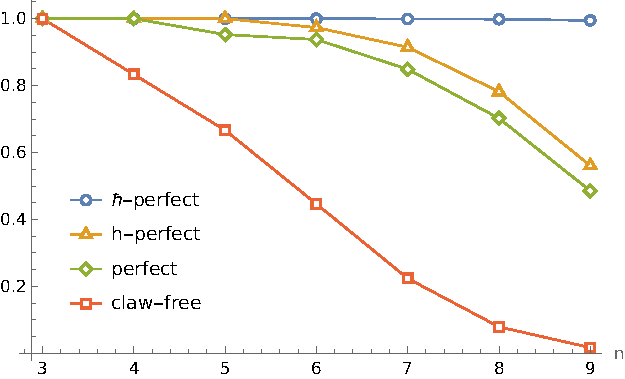
\includegraphics[width=0.45\textwidth]{percentage_new.pdf}
    \caption{The percentages of claw-free graphs, perfect graphs, $h$-perfect graphs and $\hbar$-perfect graphs in all connected graphs for the fixed number $n$ of vertices.}
    \label{fig:percentage}
\end{figure}

The procedure for determining the number of $\hbar$-perfect graphs on $8$ and $9$ vertices, respectively, is as follows. Based on the fact that the graph $G_{15}$ introduced in Appendix~\ref{ssec:hper2} is $\hbar$-perfect, we can use Property~\ref{thm:subgraph2} to filter out all the $\hbar$-perfect graphs isomorphic to subgraphs of $G_{15}$.

For all the $h$-imperfect graphs with $8$ vertices, we first check whether $G$ has $\bar{C}_7$ as its induced subgraph. If this is the case, then $G$ is $\hbar$-imperfect. In total, there are $17$ graphs in this case. Otherwise, we claim that $G$ is $\hbar$-perfect in the following three cases:
\begin{enumerate}
    \item $G$ contains a pair of vertices $i$ and $j$ such that $j$ is either a copy or a split of $i$;
    \item $G$ is a fully connected join of the other two graphs;
    \item All the normal vectors of the facets of ${\rm STAB}(G)$ contain $0$.
\end{enumerate}
This claim holds for the following reasons.
For convenience, we call graphs in those three cases \textit{reducible}.
In the first case, the resulting graph by removing $j$ from $G$ is $\hbar$-perfect since it cannot be $\bar{C}_7$. Properties~\ref{thm:splitting2} and \ref{thm:copy2} ensure that $G$ is also $\hbar$-perfect.
In the second case, each component is $\hbar$-perfect since it cannot be $\bar{C}_7$. Property~\ref{thm:connected_union2} ensures that $G$ is also $\hbar$-perfect.
In the third case, all facet-induced subgraphs are $\hbar$-perfect since they cannot be $\bar{C}_7$, and hence all the corresponding weighted beta numbers are equal to the weighted independence numbers. Consequently, $G$ is $\hbar$-perfect.

There are only $102$ graphs beyond those $3$ classes, $2$ among which are induced subgraphs of $G_{15}$ and hence $\hbar$-perfect. Then there are $100$ undetermined graphs, for which we apply the numerical tools and find them to be $\hbar$-perfect (up to a $<1\times10^{-5}$ gap between the lower and upper bounds), except one graph as in Fig.~\ref{fig:otherghs}(a) which is named as $G_8$.
Hence, there are $18$ $\hbar$-imperfect graphs in total for the case of $8$ vertices.

\begin{figure}[ht]
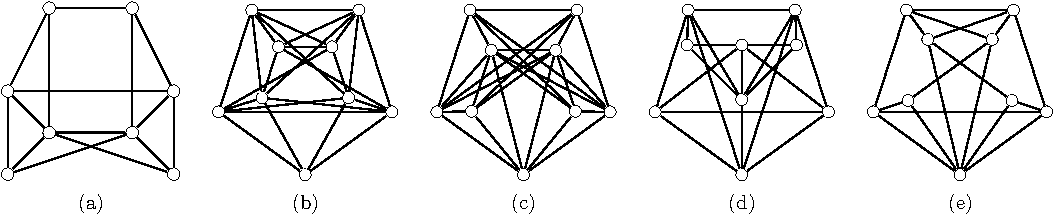
\includegraphics[width=0.9\linewidth]{basicghs.pdf}
\caption{The $\hbar$-imperfect graphs with no more than $9$ vertices which do not have other $\hbar$-imperfect graphs as induced subgraphs. Anticycles $\bar{C}_7$ and $\bar{C}_9$ are not listed here.}\label{fig:otherghs}
\end{figure}

Similarly, for all $h$-imperfect graphs with $9$ vertices, we first check whether $G$ has $\bar{C}_7$ or $G_8$ as its induced subgraphs. If this is the case, then $G$ is $\hbar$-imperfect. In total, there are $1414$ graphs in this case. Otherwise, $G$ cannot have other $\hbar$-imperfect graphs as induced subgraphs, since all $\hbar$-imperfect graphs with no more than $9$ vertices have either $\bar{C}_7$ or $G_8$ as an induced subgraph. Hence, if $G$ is reducible, then $G$ is $\hbar$-perfect.

There are only $2963$ graphs which are neither reducible nor induced subgraphs of $G_{15}$, for which we apply the numerical tools and find $2880$ ones to be $\hbar$-perfect (up to a $<1\times10^{-5}$ gap between the lower and upper bounds), $\bar{C}_9$ and other $4$ graphs as illustrated in Fig.~\ref{fig:otherghs}(b-e) to be $\hbar$-imperfect, and $78$ undetermined ones. For those $78$ undetermined ones, the gap between the upper bound of the weighted beta number and the corresponding weighted independence number is less than $3\times10^{-3}$.




\subsection{Further properties of the hierarchy}
\label{ssec:hierprop}

\begin{lemma}\label{lm:repdown}
For a given set of observables $\{S_i\}_{i=1}^n$ with a frustration graph $G$, let $S'_i = S_i\otimes M_i$ with $M_i = \otimes_{j=1}^n M_{ji}$ and $M_{ji}=Z$ if $j=i$, otherwise $M_{ji} = \id$. Then $\downarrow\hspace{-0.3em}{\cal Q}(\{S_i\}) \subseteq {\cal Q}(\{S'_i\}) \subseteq \be(G)$.
\end{lemma}
\begin{proof}
	By definition, for any point $p$ in ${\cal Q}(\{S_i\})$, it corresponds to a state $\rho$. More explicitly, the point can be represented as 
	$p = (\langle S_1\rangle_{\rho}^2, \ldots, \langle S_n\rangle_{\rho}^2)$.

	Let $\sigma = \rho \otimes (|0\rangle\langle 0|)^{\otimes n}$. The direct calculation shows that $\langle S'_i\rangle_{\sigma} = \langle S_i\rangle_{\rho}$. 
Hence,
	$p = (\langle S'_1\rangle_{\sigma}^2, \ldots, \langle S'_n\rangle_{\sigma}^2) \in {\cal Q}(\{S'_i\})$.
	Furthermore, let $\tau_x = x |0\rangle\langle 0| + (1-x)\id/2$ with $x\in [0,1]$, and $\sigma_{\vec{x}} = \rho\otimes(\otimes_{i=1}^n \tau_{x_i})$. Then we have $\langle S'_i\rangle_{\sigma_{\vec{x}}} = x_i \langle S_i\rangle_{\rho}$ which results in the point $p_{\vec{x}} = (x_1^2 \langle S_1\rangle_{\rho}^2, \ldots, x_n^2 \langle S_n\rangle_{\rho}^2)$. By varying the coefficient vector $\vec{x}$, we can obtain any point elementwise no more than $p$. That is, all those points are in ${\cal Q}(\{S'_i\})$. Consequently, we conclude that $\downarrow\hspace{-0.3em}{\cal Q}(\{S_i\}) \subseteq {\cal Q}(\{S'_i\})$.

 Finally, the two sets $\{S_i\}$ and $\{S'_i\}$ share the same frustration graph $G$, due to the fact that all matrices $M_i$ commute with each other. Consequently, ${\cal Q}(\{S'_i\}) \subseteq \be(G)$.
\end{proof}

\begin{theorem}
Given a graph $G$ with $n$ vertices, let $T_r$ be the projection of the feasible set of \eqref{mom} on the coordinates $\left(\langle x_i\rangle^2\right)_{i=1}^n$, that is,
\begin{equation}
    T_r\coloneqq\left\{\left(\langle x_i\rangle^2\right)_{i=1}^n\,\middle|\, M_r\succeq0, [M_r]_{1,1}=1, [M_r]_{u,v}=[M_r]_{a,b}\ (\forall\langle u^*v\rangle=\langle a^*b\rangle)\right\}.
\end{equation}
Then it holds that $\be(G) \subseteq T_r$. Besides, as $r$ goes to infinity, $T_r$ converges to $\be(G)$ in all nonnegative directions.
\end{theorem}
\begin{proof}
Let $\{S_i\}$ be any realization of the graph $G$. Then, the corresponding expectations with respect to any quantum state $\rho$ fulfill the constraints of \eqref{mom} and hence, ${\cal Q}(\{S_i\}) \subseteq T_r$.
Due to the arbitrariness of $\{S_i\}$, Lemma~\ref{lm:repdown} implies that $\downarrow\hspace{-0.3em} {\cal Q}(\{S_i\}) \subseteq T_r$. Then the convexity of $T_r$ leads to $\conv(\downarrow\hspace{-0.3em}{\cal Q}(\{S_i\})) \subseteq T_r$.
That is, $\be(G) \subseteq T_r$.

On the other hand, for each direction $w \ge 0$, the optimal value $\lambda_r(G,w)$ converges to $\beta(G,w)$. In other words, $T_r$ converges to $\be(G)$ in each nonnegative direction.
\end{proof}

\begin{theorem}
	The following program with $\lambda_r(G,w)$ defined in Eq.~\eqref{mom} is equivalent to an SDP:
\begin{align}\label{eq:deltaapp_inappendix}
	\omega_r \coloneqq\ &\max \sum\nolimits_i w_i\nonumber\\
	{\rm s.t.}\ & \lambda_r(G,w) \le 1,\nonumber\\
	     & w\ge 0.
\end{align}
\end{theorem}
\begin{proof}
Notice that the SDP in Eq.~\eqref{mom} can be reformulated as
\begin{align}\label{eq:original}
	\lambda_r(G,w) =\ &\sup \sum\nolimits_{i=1}^n w_i y_i\nonumber\\
	{\rm s.t.}\ & M_r = A_0 + \sum\nolimits_{j=1}^k y_j A_j \succeq 0,
\end{align}
where $A_j$'s are appropriate constant matrices encoding the equivalence relations and the Hermitian property of $M_r$ in Eq.~\eqref{mom}, and $A_0$ is the matrix with $[A_0]_{1,1}=1$ and all other elements being $0$. 
Then the dual SDP of Eq.~\eqref{eq:original} is
\begin{align}\label{eq:dual}
	\tilde{\lambda}_r(G,w)	\coloneqq\ &\inf \tr(Z A_0)\nonumber\\
	{\rm s.t.}\ & \tr(ZA_i) = -w_i, \ i=1, \ldots, n, \nonumber\\
		    & \tr(ZA_i) = 0, \ i=n+1, \ldots, k,\nonumber\\
            &\ Z\succeq0.
\end{align}
With tricks similar to those in \cite{josz2016strong}, one can show that there is no duality gap between Eq.~\eqref{eq:original} and Eq.~\eqref{eq:dual}, i.e. $\tilde{\lambda}_r(G,w) = \lambda_r(G,w)$. Then, for any feasible solution $w$ to Eq.~\eqref{eq:deltaapp_inappendix}, we have $\tilde{\lambda}_r(G,w)\le1$ and hence there exists a matrix $Z$ satisfying $\tr(ZA_0) \le 1$ as well as the conditions in Eq.~\eqref{eq:dual}.
Consequently, such a pair $(w,Z)$ is feasible to the following SDP:
\begin{align}\label{eq:omega}
	\tilde{\omega}_r\coloneqq\ &\sup \sum\nolimits_{i=1}^n w_i\nonumber\\
	{\rm s.t.}\ &\tr(ZA_i) = -w_i,\ i=1,\ldots,n,\nonumber\\
		    &\tr(ZA_i) = 0,\ i=n+1,\ldots,k,\nonumber\\
		    &\tr(ZA_0) \le 1,\nonumber\\
		    &\ w_i \ge 0,\quad Z\succeq0.
\end{align}
Conversely, any feasible solution $(w,Z)$ to Eq.~\eqref{eq:omega} is also a feasible solution to Eq.~\eqref{eq:dual}, implying $\lambda_r(G,w) =\tilde{\lambda}_r(G,w)  \le 1$. Therefore, such $w$ is feasible to Eq.~\eqref{eq:deltaapp_inappendix}. We thus conclude that $\omega_r = \tilde{\omega}_r$ and finish the proof.
\end{proof}
\subsection{Asymptotic prevalence of $\hbar$-imperfectness}
\label{ssec:asym}
\begin{theorem}
	The number of $\hbar$-perfect graphs with $n\gg 1$ vertices is at most $2^{c n(n-1)/2}$ for some constant $c<1$.
\end{theorem}
\begin{proof}
	Here we utilize the Erd\"{o}s-R\'{e}nyi random graph model, $G(n,p)$. In this model, there are $N = n(n-1)/2$ potential edges in $G(n,p)$, each of which is included with an independent and identical probability $p$. 

	We define a function $f(X_1, \ldots, X_N)$ as the number of induced subgraphs of $G(n,p)$ that are isomorphic to a specific $\hbar$-imperfect graph, $H_k$, on $k$ vertices, e.g., the anti-cycle graph $\bar{C}_7$ on $7$ vertices. 
	Notice that there are $C(n,k)$ ways to choose a subgraph on $k$ vertices from the random graph $G(n,p)$ on $n$ vertices, each of which is again a random graph $G(k,p)$. Thus, the expectation of $f(X_1, \ldots, X_N)$ is given by:
\begin{equation}
	\langle f(X_1, \ldots, X_N) \rangle = p_0\, C(n,k),
\end{equation}
where $p_0$ is the probability that the random graph $G(k,p)$ with $k$ vertices is isomorphic to $H_k$.

For an instance of the random graph to be $\hbar$-perfect, it must not contains any induced subgraph isomorphic to $H_k$, which means that the corresponding value of $f(X_1,\ldots,X_N)$ is $0$. Besides, the change in $f(X_1,\ldots,X_N)$ when the adjacent relation between two vertices switches is at most $c_e = C(n-2,k-2)$, since this operation can affect at most $c_e$ induced subgraphs containing these two vertices. Applying McDiarmid's inequality, we obtain the following upper bound on the probability of $f(X_1,\ldots,X_N) = 0$:
\begin{equation}\label{eq:mcd_ineq}
\begin{aligned}
	\text{Pr}\{f=0\} \le& \text{Pr}\{f\le \langle  f\rangle - p_0 C(n,k)\}\\
	\le& \exp({-2p_0^2 C(n,k)^2/[N c_e^2]})\\
	=& \exp({-2p_0^2 N/C(k,2)^2}),
\end{aligned}
\end{equation}
where the second inequality is due to McDiarmid's inequality ${\rm Pr}\{f\le \langle f\rangle - \epsilon\} \le \exp(-2\epsilon^2/[N c_e^2])$ with $\epsilon=p_0\, C(n,k)$ and $c_e$ being the upper bound of change in $f$ for the switch of each $X_i$.

For the case of $p = 1/2$, the expression in Eq.~\eqref{eq:mcd_ineq} represents the ratio of $\hbar$-perfect graphs to the total number of graphs, that is, $2^N$. The resulting number of $\hbar$-perfect graphs is upper bounded by $2^N  \exp(-{2p_0^2 N/C(k,2)^2} ) = 2^{c  N}$, with the constant $c$ given by
$1 - 2 p_0^2 \log e/C(k,2)^2$.
Since $p_0 > 0$, by setting $k$ to any number not less than $7$, it is clear that $c < 1$.
\end{proof}



\section{Applications}
\label{sec:app2}
\subsection{Entanglement detection and estimation}
\label{ssec:entanglement}
Here we use the Euclidean distance $d(\rho)$ from the point $\{\langle O_i\rangle\}$ to {$\be(G)$, with $G$ the frustration graph of Pauli strings $\{O_i\}$}, to provide a lower bound of ${\cal E}_{\rm HS}(\rho)$, i.e., the entanglement measured by the Hilbert-Schmidt distance~\cite{witte1999new}:
\begin{equation}
    {\cal E}_{\rm HS}(\rho) \coloneqq \min_{\sigma \in {\rm SEP}} (\tr[(\rho-\sigma)^2])^{1/2},
\end{equation}
with ${\rm SEP}$ stands for the set of separable states.

Since $\be(G)$ is a superset of the set of all points generated from separable states with the same observables $\{O_i\}$, for any separable state $\sigma$, it holds that
\begin{align}
	d^2(\rho) &= \min_{p\in \be(G)} \sum_i ||\langle O_i\rangle_{\rho}| - p_i |^2 \nonumber\\
    &\le \sum\nolimits_i ||\langle O_i\rangle_{\rho}| - |\langle O_i\rangle_{\sigma}| |^2 \nonumber\\
            &\le \sum\nolimits_i |\langle O_i\rangle_{\rho} - \langle O_i\rangle_{\sigma} |^2 \nonumber\\
	    &= \sum\nolimits_i (\tr[O_i (\rho - \sigma)])^2 \nonumber\\
	    &= \tr\big[ \big(\sum\nolimits_i O_i\otimes O_i\big) (\rho-\sigma)\otimes(\rho-\sigma)  \big]\nonumber\\
	    &\le \Big(\tr\big[ \big(\sum\nolimits_i\! O_i\otimes O_i\big)^2\big] \tr\big[ (\rho-\sigma)^2\otimes(\rho-\sigma)^2  \big] \Big)^{\frac{1}{2}}\nonumber\\
	    &\le \Big(\tr\big[ \big(\sum\nolimits_i O_i\otimes O_i\big)^2\big] \Big)^{\frac12}\tr\big[ (\rho-\sigma)^2\big] ,
\end{align}
which implies that
\begin{equation}
	{\cal E}_{\rm HS}(\rho) \ge d(\rho) / \Big(\tr\big[ \big(\sum\nolimits_i O_i\otimes O_i\big)^2\big] \Big)^{\frac{1}{4}}.
\end{equation}

For convenience, we relabel the four $2$-dimensional Bell states as
\begin{align}
	|\Psi_1\rangle = (|00\rangle+|11\rangle)/\sqrt{2},\,
	|\Psi_2\rangle = (|00\rangle-|11\rangle)/\sqrt{2}, \nonumber\\
	|\Psi_3\rangle = (|01\rangle+|10\rangle)/\sqrt{2},\,
	|\Psi_4\rangle = (|01\rangle-|10\rangle)/\sqrt{2}.
\end{align}
Then, by representing the $2^k$-dimensional space by $k$ qubits, we obtain the $4^k$ maximally entangled states represented by 
\begin{equation}
	|\Psi_{\vec{t}}\rangle_{1,\ldots,2i-1;2,\ldots,2i} \coloneqq \otimes_{i=1}^k |\Psi_{t_i}\rangle_{2i-1,2i},
\end{equation}
where $t_i \in \{1, 2, 3, 4\}$, $|\Psi_{t_i}\rangle_{2i-1,2i}$ is the maximally entangled state $|\Psi_{t_i}\rangle$ between the particles $2i-1$ and $2i$, the particles with odd labels belong to the first party, and those with even labels belong to the second party.

Denote by $\{\sigma_j\}_{j=0}^3$ the Pauli matrices $I, X, Y, Z$ in order.
Notice that $|\Psi_t\rangle$ is the common eigenstate of $\{\sigma_j\otimes\sigma_j\}_{j=0}^3$ with the eigenvalue being $\pm 1$ for any $t\in \{1,2,3,4\}$.
This implies that the state $|\Psi_{\vec{t}}\rangle$ is the common eigenstate of $\{S_l\otimes S_l\}_{l=0}^{4^k-1}$ with eigenvalues being $\pm 1$ for any $\vec{t}$, where $S_l$ is the Pauli string $\otimes_{i=1}^k \sigma_{l_i}$ and $l_i$ is the $i$-th digit of $l$ in the base of $4$.
Hence, $|\langle \Psi_{\vec{t}}| S_l\otimes S_l|\Psi_{\vec{t}}\rangle| = 1$, $\forall l$, which is impossible for separable states. Here we take $k=2$ as an example. Denote by $G$ the frustration graph of the $15$ operators $\{S_l\}_{l=1}^{15}$ by omitting the identity $S_0$, then $\beta(G)=3$. Thus, for any separable state $\sigma$, $\sum_{l=1}^{15} |\langle S_l\otimes S_l\rangle_{\sigma}| \le 3$.
\begin{theorem}
	For any Bell diagonal state $\rho = \sum_{i=1}^4 p_i |\Psi_i\rangle\langle \Psi_i|$ with $\sum_{i=1}^4 p_i = 1$ and $p_i \ge 0$, it is entangled if and only if $p({\cal S}, {\cal S}', \rho)$ is outside the set $\{(x,y,z)|x+y+z\le 1\} \cap \mathbb{R}^3_+$, where ${\cal S} = {\cal S'} = \{X, Y, Z\}$.
\end{theorem}
\begin{proof}
An known necessary and sufficient condition for $\rho$ to be entangled is $\max_i p_i > 1/2$. Without loss of generality, we assume that $p_1 \ge p_2 \ge p_3 \ge p_4$.
Notice that
\begin{align}
	|\Psi_1\rangle\langle \Psi_1| = (\id + XX - YY + Z Z)/4, \ 
	|\Psi_2\rangle\langle \Psi_2| = (\id - XX + YY + Z Z)/4, \nonumber\\
	|\Psi_3\rangle\langle \Psi_3| = (\id + XX + YY - Z Z)/4, \ 
	|\Psi_4\rangle\langle \Psi_4| = (\id - XX - YY - Z Z)/4.
\end{align}
The state $\rho$ can be reformulated as
\begin{equation}
	\rho = [\id + (p_1+p_3-p_2-p_4)XX + (p_2+p_3-p_1-p_4)YY + (p_1+p_2-p_3-p_4)Z Z]/4.
\end{equation}
Then the condition that $p({\cal S}, {\cal S}', \rho)$ is in the set $\{(x,y,z)|x+y+z\le 1\} \cap \mathbb{R}^3_+$  is equivalent to
\begin{equation}
	|p_1+p_3-p_2-p_4| + |p_2+p_3-p_1-p_4| + |p_1+p_2-p_3-p_4| \le 1.
\end{equation}
Under the assumption that $p_1\ge p_2 \ge p_3 \ge p_4$, it can be simplified to
\begin{align}
	1 &\ge p_1+p_3-p_2-p_4 + |p_1+p_4 - p_2 -p_3| + p_1 + p_2 - p_3 -p_4\nonumber\\
	  &= p_1+p_3-p_2-p_4 + |p_1+p_4 - p_2 -p_3| + p_1 + p_2 - p_3 -p_4\nonumber\\
	  &= 2p_1-2p_4 + |p_1+p_4-p_2-p_3|\nonumber\\
	  &= \max \{4p_1-1,1-4p_4\},
\end{align}
which is equivalent to $1/2 \ge p_1 = \max_i p_i$, i.e., $\rho$ is not entangled.
\end{proof}
We continue to consider the multipartite entanglement exemplified by GHZ states.
Let
\begin{align}
|\text{GHZ}_1\rangle = (|000\rangle + |111\rangle)/\sqrt{2},
|\text{GHZ}_2\rangle = (|000\rangle - |111\rangle)/\sqrt{2},\nonumber\\
|\text{GHZ}_3\rangle = (|100\rangle + |011\rangle)/\sqrt{2},
|\text{GHZ}_4\rangle = (|100\rangle - |011\rangle)/\sqrt{2},\nonumber\\
|\text{GHZ}_5\rangle = (|010\rangle + |101\rangle)/\sqrt{2},
|\text{GHZ}_6\rangle = (|010\rangle - |101\rangle)/\sqrt{2},\nonumber\\
|\text{GHZ}_7\rangle = (|110\rangle + |001\rangle)/\sqrt{2},
|\text{GHZ}_8\rangle = (|110\rangle - |001\rangle)/\sqrt{2}.
\end{align}
\begin{theorem}
	For any tripartite GHZ diagonal state $\rho = \sum_{i=1}^8 p_i |{\rm GHZ}_i\rangle\langle {\rm GHZ}_i|$ with $\sum_{i=1}^8 p_i = 1$ and $p_i\ge 0$, it is genuinely tripartite entangled if and only if  $\sum_{i=1}^7 |\langle O_i\rangle_{\rho}| > 3$, where $O_i$ are  
\begin{equation}\label{eq:stabilizer_inappendix}
	Z Z\id, Z\id Z, \id Z Z, XXX,-YYX, -YXY, -XYY.
\end{equation}
\end{theorem}
\begin{proof}
	It is known that $\rho$ is genuinely tripartite entangled if and only if $\max_i p_i > 1/2$. We first prove that the fact that $\rho$ is genuinely tripartite entangled implies $\sum_{i=1}^7 |\langle O_i\rangle_{\rho} | > 3$.

	Without loss of generality, we assume that $p_1 = \max_i p_i$, since all the $8$ GHZ states can be changed to each other via local unitaries, which does not affect entanglement.
	Notice that 
	\begin{equation}
		|{\rm GHZ}_1\rangle\langle {\rm GHZ}_1| = \big(\id_8 + \sum\nolimits_{i=1}^7 O_i\big)/8.
	\end{equation}
	Hence,
	\begin{equation}
		p_1 = \langle {\rm GHZ}_1|\rho|{\rm GHZ}_1\rangle = \big(1 + \sum\nolimits_{i=1}^7 \langle O_i\rangle_{\rho}\big)/8 > 1/2
	\end{equation}
	is equivalent to $\sum\nolimits_{i=1}^7 \langle O_i\rangle_{\rho} > 3$ and this implies that $\sum\nolimits_{i=1}^7 |\langle O_i\rangle_{\rho}| > 3$.

	Besides, whenever $\rho$ is not genuinely tripartite entangled, we know that $\sum\nolimits_{i=1}^7 |\langle O_i\rangle_{\rho}| \le 3$.
	Consequently, $\rho$ is genuinely tripartite entangled if and only if $\sum\nolimits_{i=1}^7 |\langle O_i\rangle_{\rho}| > 3$.
\end{proof}
As for the high-dimensional case, we use the following embedding technique when the dimension is not a power of $2$. Here we take the $3$-dimensional case to illustrate the idea.
Denote by $X^{(i)}, Y^{(i)}, Z^{(i)}$ the operators $X, Y, Z$ in the two-dimensional subspace without the $i$-th dimension. Then it holds for any separable state $\rho$  that
\begin{equation}\label{eq:subineq}
	\sum_{i,j=1}^3 \big[ |\langle X^{(i)} X^{(j)}\rangle_{\rho}| + |\langle Y^{(i)} Y^{(j)}\rangle_{\rho}| + |\langle Z^{(i)} Z^{(j)}\rangle_{\rho}|\big] \le 4.
\end{equation}
\begin{proof}
	Let $P_i = \id_3 - |i\rangle\langle i|$, $\rho_{ij} = (P_i\otimes P_j) \rho (P_i\otimes P_j) /\tr(P_i\otimes P_j \rho)$ if $\tr(P_i\otimes P_j \rho) \neq 0$. Otherwise, let $\rho_{ij} = \id_4/4$ the $4$-dimensional maximally mixed state. 
	By definition, $\rho_{ij}$ is a bipartite state with local dimensions being $2$. If $\rho$ is a separable state with the decomposition
	\begin{equation}
		\rho = \sum_k p_k \rho_{A,k} \otimes \rho_{B,k}.
	\end{equation}
	Then we have that
	\begin{equation}
		\rho_{ij} = \sum_k p_k (P_i\rho_{A,k}P_i) \otimes (P_j\rho_{B,k}P_j)/\tr(P_i\otimes P_j \rho)
	\end{equation}
	separable, too.
	This leads to
	\begin{equation}
		|\langle XX\rangle_{\rho_{ij}}|
		+|\langle YY\rangle_{\rho_{ij}}|
		+|\langle ZZ\rangle_{\rho_{ij}}| \le 1,
	\end{equation}
	which is equivalent to
\begin{equation}
	|\langle X^{(i)} X^{(j)}\rangle_{\rho}| + |\langle Y^{(i)} Y^{(j)}\rangle_{\rho}| + |\langle Z^{(i)} Z^{(j)}\rangle_{\rho}| \le \tr(P_i\otimes P_j \rho).
\end{equation}
Consequently,
\begin{equation}
	\sum_{i,j=1}^3 |\langle X^{(i)} X^{(j)}\rangle_{\rho}| + |\langle Y^{(i)} Y^{(j)}\rangle_{\rho}| + |\langle Z^{(i)} Z^{(j)}\rangle_{\rho}| \le \sum_{i,j=1}^3 \tr(P_i\otimes P_j \rho) = 4.
\end{equation}
\end{proof}
We first consider the state
\begin{equation}
    \rho(p) = (1-p) |\Psi_3\rangle\langle \Psi_3| + p |\Phi'\rangle\langle \Phi'|,
\end{equation}
where $|\Psi_3\rangle = (\sum_{i=1}^3 |ii\rangle)/\sqrt{3}$ and $|\Phi'\rangle = (|12\rangle + |21\rangle)/\sqrt{2}$. 
Direct calculation shows that the value of the left-hand side of Eq.~\eqref{eq:subineq} is
\begin{equation}
\frac{2}{3}(2 | 2-5 p| -5 p+8),
\end{equation}
whose minimum is $4$ and can only be achieved with $p=2/5$.

Then we consider a state that is entangled but unfaithful~\cite{Weilenmann2019EntanglementDB},
\begin{equation}
	\rho = 0.999 (0.50179 |\phi_1\rangle\langle \phi_1| + 0.49821|\phi_1\rangle\langle \phi_1|) + 0.001 \id/9,
\end{equation}
where
\begin{align}
	|\phi_1\rangle &= 0.628|11\rangle - 0.778 |22\rangle,\nonumber\\
	|\phi_2\rangle &= 0.807|01\rangle - 0.185|02\rangle  - 0.102 |10\rangle - 0.027|11\rangle + 0.011|12\rangle + 0.551|20\rangle - 0.024|21\rangle - 0.022|22\rangle.
\end{align}
Direct calculation shows that the value of the left-hand side of Eq.~\eqref{eq:subineq} is $4.8514 > 4$, i.e., a violation of the bound for separable states.
\subsection{Sample complexity in shadow tomography}\label{ssec:tomography}
\begin{theorem}
  Let ${\cal D}$ be the set of probability distributions and let $\alpha^*(G)$ and $\vartheta(G)$ be the fractional packing number~\cite{schrijver1979fractional} and the Lov\'{a}sz number~\cite{lovasz1979shannon} of graph $G$, respectively. It holds
  \begin{equation}
    \min_{w\in {\cal D}} \beta(G,w) \in [1/\alpha^*(\bar{G}), 1/\vartheta(\bar{G})],
  \end{equation}
where the lower bound is achieved whenever $G$ is $\hbar$-perfect.
\end{theorem}
\begin{proof}
  It is known that
  \begin{equation}
    \beta(G,w) \in [\alpha(G,w), \vartheta(G,w)],\, \forall w \in {\cal D}.
  \end{equation}
  We continue to prove that
  \begin{align}
    \min_{w\in{\cal D}} \alpha(G,w) &= 1/\alpha^*(\bar{G}),\label{eq:alphastar}\\
    \min_{w\in{\cal D}} \vartheta(G,w) &= 1/\vartheta(\bar{G}).
  \end{align}
  For $G$ to be $\hbar$-perfect, we have $\alpha(G,w) = \beta(G,w), \forall w\ge 0$, which implies that the lower bound is exact together with Eq.~\eqref{eq:alphastar}.
  Notice that
  \begin{align}
    \min_{w\in {\cal D}} \alpha(G,w) = \min_{w\ge 0} \frac{\alpha(G,w)}{\sum_i w_i}
                                     = \min_{w\ge 0, \alpha(G,w)=1} \frac{1}{\sum_i w_i}
                                     = \frac{1}{\alpha^*(\bar{G})},
  \end{align}
  where the last line is due to the definition of $\alpha^*(\bar{G})$~\cite{schrijver1979fractional}, i.e.,
  \begin{align}
    \alpha^*(G) \coloneqq \max &\quad\sum_i w_i\nonumber\\
    \mathrm{s.t.}&\quad w\ge 0,\nonumber\\
         &\quad\sum_{i\in C} w_i \le 1, \,\forall C \in {\rm Clis },
  \end{align}
  with ${\rm Clis}$ being the set of cliques of $\bar{G}$, or equivalently, the set of independence sets of $G$.

  Similarly,
  \begin{align}
    \min_{w\in {\cal D}} \vartheta(G,w) = \min_{w\ge 0} \frac{\vartheta(G,w)}{\sum_i w_i} = \min_{w\ge 0, \vartheta(G,w)=1} \frac{1}{\sum_i w_i} = \frac{1}{\vartheta(\bar{G})},
  \end{align}
  where the last line is due to the fact that~\cite{knuth1994sandwich}
  \begin{align}
                                     & {\max_{w\ge 0, \vartheta(G,w)=1} \sum_i w_i}\nonumber\\
  =& {\max_{w\ge 0, \sum_i w_i v_i\le 1, \forall v\in {\rm TH}(G)} \sum_i w_i}\nonumber\\
                                     =& {\max_{w\in {\rm TH}(\bar{G})} \sum_i w_i}\nonumber\\
                                     =& \,\vartheta(\bar{G}),
  \end{align}
  since
  \begin{equation}
  {\rm TH}(\bar{G}) = \{w\mid w\ge 0, \sum_i w_i v_i \le 1, \forall v \in {\rm TH}(G)\}.
  \end{equation}
\end{proof}

\begin{lemma}
  $\beta(G,w)$ is a convex function of $w \ge 0$.
\end{lemma}
\begin{proof}
  By definition, for any $w\ge 0, \tilde{w}\ge 0$ and $x\in [0,1]$, we have
  \begin{align}
   & \,\beta(G,x w + (1-x) \tilde{w})\nonumber\\ 
    =& \max_{\rho}[x \sum_i w_{i} \langle S_i\rangle_{\rho}^2 + (1-x) \sum_i \tilde{w}_{i} \langle S_i\rangle_{\rho}^2]\nonumber\\
    \le& \,x\max_{\rho} \sum_i w_{i} \langle S_i\rangle_{\rho}^2 + (1-x) \max_{\rho}\sum_i \tilde{w}_{i} \langle S_i\rangle_{\rho}^2\nonumber\\
    =& \,x \beta(G,w) + (1-x)\beta(G,\tilde{w}).
  \end{align}
\end{proof}
\begin{theorem}
Denote ${\cal D}$ the set of all probability distributions and ${\cal D}_s$ the set of the ones which has the symmetry induced by graph $G$, then
  \begin{equation}
    \min_{w\in {\cal D}} \beta(G,w) = \min_{w\in {\cal D}_s} \beta(G,w),
  \end{equation}
  Especially, when $G$ is vertex-transitive, $\min_{w\in {\cal D}} \beta(G,w) = \beta(G)/n$ with $n$ being the number of vertices of $G$.
\end{theorem}
For example, all cycle graphs and their complements are vertex-transitive. For a given cycle graph $C_n$ with $n$ vertices, $\beta(C_n) = \alpha(C_n) = \lfloor n/2 \rfloor$~\cite{xu2023bounding}. Thus, the sample complexity parameter $\delta$ is $\beta(C_n)/n = \lfloor n/2 \rfloor/n \approx 1/2$ when $n$ is large enough. 
For a given anti-cycle graph $\bar{C}_n$ with $n$ vertices, $2= \alpha(\bar{C}_n) < \beta(\bar{C}_n) \le \vartheta(\bar{C}_n)$, where $\vartheta(\bar{C}_n) = 1+1/\cos(\pi/n)$ when $n$ is odd and $\vartheta(\bar{C}_n) = 2$ when $n$ is even~\cite{lovasz1979shannon}. Thus, $\beta(\bar{C}_n)\approx 2$ and the sample complexity parameter $\delta$ is $\beta(\bar{C}_n)/n \approx 2/n$ when $n$ is large enough. Since the sample complexity is in $[\Omega(1/[\epsilon^2 \delta]), O(\log n/[\epsilon^2 \delta])]$ for the precision $\epsilon$, the sample complexity for the anti-cycle $\bar{C}_n$ is higher than the one for the cycle $C_n$. More explicitly, the ratio is at least $\Omega(n/\log n)$ for the same precision.

For a random graph $G(n,p)$ with $n$ vertices and $p$ is the probability of each edge~\cite{coja2005lovasz}, its complement graph is $G(n,1-p)$. Then the sample complexity for $G=G(n,p)$ is lower bounded by 
\begin{equation}
    \Omega(1/[\epsilon^2 \delta]) = \Omega(\vartheta(\bar{G})/\epsilon^2)  = \Omega(\vartheta(G(n,1-p))/\epsilon^2) = \Omega(\sqrt{n/(1-p)}/\epsilon^2),
\end{equation}
where the last equality is from Theorem~4 in Ref.~\cite{coja2005lovasz}.




\subsection{Using classical graph algorithms for bounding ground state energies}\label{ssec:ground}
For a sequence of real-valued coefficients $a_i$, let $H=\sum_i a_i A_i$ be a Hamiltonian. 
It is a central, but at the same time very difficult, task to find or estimate the smallest or the highest energy of $H$ generally. Given $\beta(G,w)$ such an estimate from the outside, this is the direction not covered by variation methods, can be established. 
We have \cite{xu2023bounding}
\begin{align}
    \label{eq:approx2_inappendix}
   \sup_\rho \langle H \rangle_\rho  &\leq \sqrt{\inf_w  \Big( \sum_i a_i^2/w_i\Big)\beta(G,w)},
\end{align}
which is equivalent to 
\begin{align}
    \label{eq:approx2__inappendix2}
   \sup_\rho \langle H \rangle_\rho  &\leq \sqrt{\inf_{w, \beta(G,w)= 1}   \sum_i a_i^2/w_i}\nonumber\\
   &= \sqrt{\inf_{w, \beta(G,w)\le 1}   \sum_i a_i^2/w_i},
\end{align}
where the last equality is from the fact that the infimum is obtained when $\beta(G,w)=1$ in the region that $\beta(G,w)\le 1$.

Here, having a $\hbar$-perfect graph again simplifies the optimization over $w$ in the above to an optimization over the stable set polytope.
To find the upper bound in Eq.~\eqref{eq:approx2_inappendix}, it is equivalent to considering the following optimization problem:
\begin{align}
    \label{eq:approx3_inappendix}
    \inf_w   &\quad\sum_i a_i^2/w_i\nonumber\\
    \mathrm{s.t.} &\quad \sum_{i\in I} w_i \le 1,\, \forall I \in {\cal I},\nonumber\\
    & \quad w_i \ge 0,
\end{align}
where ${\cal I}$ contains all independence sets of $G$.
It is clear to see that all the constraints in Eq.~\eqref{eq:approx3_inappendix} are linear. Besides, $\sum_i a_i^2/w_i$ is a convex function of $w$ since $1/w_i$ is a convex function of $w_i$ for $w_i>0$. Consequently, the programming in Eq.~\eqref{eq:approx3_inappendix} is a convex program with linear constraints, which in principle can be solved efficiently.



Here, we consider the following model as an example:
\begin{equation}
H_n =	a X_1+b Z_1 + c Y_{n} + \sum_{i=1}^{n-1}(d_i X_iX_{i+1} + e_i Z_iZ_{i+1}),
\end{equation}
with coefficients $u = (a,b,c,d_1,\ldots,d_{n-1},e_1,\ldots,e_{n-1})$.

The frustration graph of the Pauli strings in $H_n$ is the cycle graph $C_{2n+1}$, which is $h$-perfect and hence $\hbar$-perfect. Then we have
\begin{align}
	\langle H_n \rangle^2 \le \inf_{w\ge 0}\sum_i u_i^2 /w_i \alpha(C_{2n+1},w) \le n\sum_i u_i^2,
\end{align}
where the last inequality holds since we simply set $w_i=1$.
In the case that $u_i=1$, that is, all coefficients are $1$, $\langle H_n\rangle \ge -\sqrt{n(2n+1)}$. 
For $n\in \{2,3,4,5,6\}$, we calculate numerically the ground state energy and compare it with the estimation. The ratio of the estimation over the exact value is
\begin{equation}
1.02749, 1.02943, 1.01672, 1.00589, 1.00416, 1.00121
.\end{equation}
The difference between the estimation and the exact value is
\begin{equation}
0.0845941, 0.13099, 0.0986868, 0.0434194, 0.036549, 0.0123609
.\end{equation}
As $n$ increases, the ratio tends to $1$ and the difference tends to $0$.

Another model is 
\begin{equation}
	\tilde{H}_n =	a X_1+b Z_1 + c Y_{n} + \sum_{i=1}^{n-1}(d_i X_iX_{i+1} + e_i Y_iY_{i+1} + f_i Z_iZ_{i+1}),
\end{equation}
with coefficients $u = (a,b,c,d_1,\ldots,d_{n-1},e_1,\ldots,e_{n-1},f_1,\ldots,f_{n-1})$.
As confirmed by direct calculation, the corresponding frustration graph is also $h$-perfect for $n\le 5$. Hence, there is also a convex program for the estimation of its ground state energy. We use the case of $n=2$ to illustrate the idea of obtaining the weight vector $w$ for a tighter bound. The idea is to increase the components of $w$ without increasing the weighted independence number. 
Let
\begin{equation}
	\tilde{H}_2 = X_1 + Z_1 + Y_2 + \left( X_1X_2 + Y_1Y_2 + Z_1Z_2 \right).
\end{equation}
Let $G$ be the frustration graph of the Pauli strings in $\tilde{H}_2$ in order.
Then
\begin{align}
	\langle \tilde{H}_2\rangle^2 \le \inf_{w\ge 0} \sum_{i=1}^6 1/w_i \beta(G,w) \le 6 \beta(G) = 18.
    \end{align}
However, by taking $w=(2,2,1,1,1,1)$, $\beta(G,w) = \beta(G)=3$ while $\sum_{i=1}^6 1 /w_i = 5$. This provides a tighter bound $\langle \tilde{H}_2\rangle^2 \le 15$. In comparison, the exact ground state energy is $-3.722935$, while the estimated lower bound is $-\sqrt{15} \approx -3.872983$, which is better than the one $-\sqrt{18} \approx -4.242641$. 

As far as we know, there is also a numerical method based on SDP relaxations to provide lower bounds on the ground state energy~\cite{wang2024certifying}. However, such a method is feasible for middle- and large-scale models only if there are lots of symmetries in the model, which ensures that a good enough estimation can be obtained within reasonable computational resources. In comparison, the graph-theoretic method still works even if there is not enough symmetry in the model at the price of precision, due to the relaxation from the Cauchy-Schwarz inequality. Notice that the symmetry in the model can also be employed to reduce the complexity in the calculation of weighted independence numbers, and hence speed up the graph-theoretic estimation.


\subsection{Quantum encoding of the independence number}\label{ssec:alpha}
\begin{theorem}
    Let a graph with $n$ vertices be encoded in $l=1/2 \log_2(n/c)$ qubits. Assume weights normalized by $\Vert w \Vert_1=n$. Then, the maximal eigenvalue of $\tilde{H}_S^{(m)}$ approximates $\beta(G,w)$ by 
    \begin{align}\label{eq:definetti-without-proj}
        \beta(G,w) \leq \lambda_{\max}\left( \tilde{H}_S^{(m)} \right) \leq \beta(G,w) + n\sqrt{ \frac{\log(n)-\log(c)}{m}}.
    \end{align}
 That is, we obtain a linear Hamiltonian encoding of the number $\beta(G,w)$ with an additive regularized error 
    \begin{align}
        \varepsilon =\left|\lambda_{\max}(\tilde{H}_S^{(m)})/n -\beta(G,w)/n\right|
    \end{align}
    by using $L$ qubits with
    \begin{align}
        L=(m+2)l\sim  O\left(\frac{\log(n/c)^2 }{\varepsilon^2}\right).
    \end{align}
\end{theorem}
\begin{proof}
Our system $\mathcal{H}_L$ under consideration consists of $L=(m+2)l$ qubits which we will consistently regard as a tensor product $\mathcal{H}_l^{(m+2)}$ of $(m+2)$ copies of a system $\mathcal{H}_l = \mathbb{C}^{2^l}$. We will refer to each factor of type $\mathcal{H}_l$ as a local system.  

Let $\rho_{\max}$ be a state on such $L$ qubits that attains the maximal eigenvalue of  $\tilde{H}_S^{(m)}$. 
W.l.O.g. we assume that $\rho_{\max}$ inherits the permutation invariance from  $\tilde{H}_S^{(m)}$. 
We start by decomposing the maximal eigenvalue as
\begin{equation}
\lambda_{\max}\bigl(\tilde{H}_S^{(m)}\bigr)
= \tr\Bigl(\tilde{H}_S^{(m)}\rho_{\max}\Bigr)
= \tr\Bigl(\tilde{H}_S^{(m)}\bigl(\rho_{\max}-\!\!\int \sigma^{\otimes (m+2)}\,d\mu(\sigma)\bigr)\Bigr)
  + \tr\Bigl(\tilde{H}_S^{(m)}\!\int \sigma^{\otimes (m+2)}\,d\mu(\sigma)\Bigr).
\end{equation}
Since $\tilde{H}_S^{(m)}$ is a composition of ${m+2 \choose 2}n$ Pauli strings acting only on two local factors and each Pauli string $S$ corresponds to a measurement with two outcomes, it follows that
\begin{equation}
\tr\bigl(S(\rho_{\max}-\!\!\int \sigma^{\otimes (m+2)}\,d\mu(\sigma))\bigr)
= \tr\bigl(S^{(2)}(\rho^{(2)}_{\max}-\!\!\int \sigma^{\otimes 2}\,d\mu(\sigma))\bigr)
\le \bigl\lVert\rho^{(2)}_{\max}-\!\!\int \sigma^{\otimes 2}\,d\mu(\sigma)\bigr\rVert_{\mathrm{LOCC}_1},
\end{equation}
where $\bigl\lVert \tau\bigr\rVert_{\mathrm{LOCC}_1} = \max_{\{M_i\}\in \mathrm{LOCC}_1} \bigl\lVert \sum_i \tr(M_{i}\tau)|i\rangle\langle i| \bigl\lVert_1$ with $\mathrm{LOCC}_1$ being the set of one-way LOCC measurement~\cite{li2015quantum}, 
$S^{(2)}$ denotes $S$ on its bipartite support, $\rho^{(2)}_{\max}$ denotes the bipartite reduced state on the same support, which is well-defined since $\rho$ is permutationally invariant.

Summing over the $n$ non-equivalent contributions gives
\begin{equation}
\tr\Bigl(\tilde{H}_S^{(m)}\bigl(\rho_{\max}-\!\!\int \sigma^{\otimes (m+2)}\,d\mu(\sigma)\bigr)\Bigr)
\le n\,\bigl\lVert\rho^{(2)}_{\max}-\!\!\int \sigma^{\otimes 2}\,d\mu(\sigma)\bigr\rVert_{\mathrm{LOCC}_1}.
\end{equation}
For the second term, one has
\begin{align}
\tr\Bigl(\tilde{H}_S^{(m)}\!\int \sigma^{\otimes (m+2)}\,d\mu(\sigma)\Bigr)
&= \int \tr\bigl(\tilde{H}_S^{(m)}\sigma^{\otimes (m+2)}\bigr)\,d\mu(\sigma)
= \int \tr\bigl(\tilde{H}_S\sigma^{\otimes 2}\bigr)\,d\mu(\sigma)\nonumber\\
&\leq \max_{\sigma} \tr\bigl(\tilde{H}_S\sigma^{\otimes 2}\bigr)
=\beta(G,w).
\end{align}
Combining the two inequalities, we obtain
\begin{equation}
\lambda_{\max}\bigl(\tilde{H}_S^{(m)}\bigr)
\le n\,\bigl\lVert\rho^{(2)}_{\max}-\!\!\int \sigma^{\otimes 2}\,d\mu(\sigma)\bigr\rVert_{\mathrm{LOCC}_1}
+ \beta(G,w).
\end{equation}
By the finite de Finetti theorem for one-way LOCC measurements~\cite[Thm.~1]{li2015quantum}, the $\mathrm{LOCC}_1$ distance satisfies
\begin{equation}
\bigl\lVert\rho^{(2)}_{\max}-\!\!\int \sigma^{\otimes 2}\,d\mu(\sigma)\bigr\rVert_{\mathrm{LOCC}_1}
\le \sqrt{\frac{2\ln d}{m}}
= \sqrt{\frac{2\ln(\sqrt{n/c})}{m}}
= \sqrt{\frac{\ln(n/c)}{m}},
\end{equation}
and hence
\begin{equation}
\lambda_{\max}\bigl(\tilde{H}_S^{(m)}\bigr)
\le \beta(G,w) + n\sqrt{\frac{\ln(n/c)}{m}}.
\end{equation}

On the other hand, we have 
\begin{align}
   \beta(G,w) = \max_{\sigma} \tr\bigl(\tilde{H}_S\sigma^{\otimes 2}\bigr)= \max{\sigma} \tr\bigl(\tilde{H}_S^{(m)} \sigma^{\otimes (m+2) }\bigr)
&\leq \lambda_{\max} \left( \tilde{H}_S^{(m)} \right) 
\end{align}
which completes the proof of \eqref{eq:definetti-without-proj}.
Setting 
\begin{equation}
m \le \frac{\ln(n/c)}{\epsilon^2}.
\end{equation}
in \eqref{eq:definetti-without-proj} yields 
\begin{align}
    \lambda_{\max}\bigl(\tilde{H}_S^{(m)}\bigr) - \beta(G,w) \leq n \epsilon.
\end{align}

Since $l = \log d = \log(n/c)$, the total length $L = (m+2)l$ satisfies
\begin{equation}
L = (m+2)l = O\!\left(\frac{\log^2(n/c)}{\epsilon^2}\right),
\end{equation}
which completes the proof.
\end{proof}

